



\frame{
\frametitle{Evaluation}
\begin{center}
%\only<1>{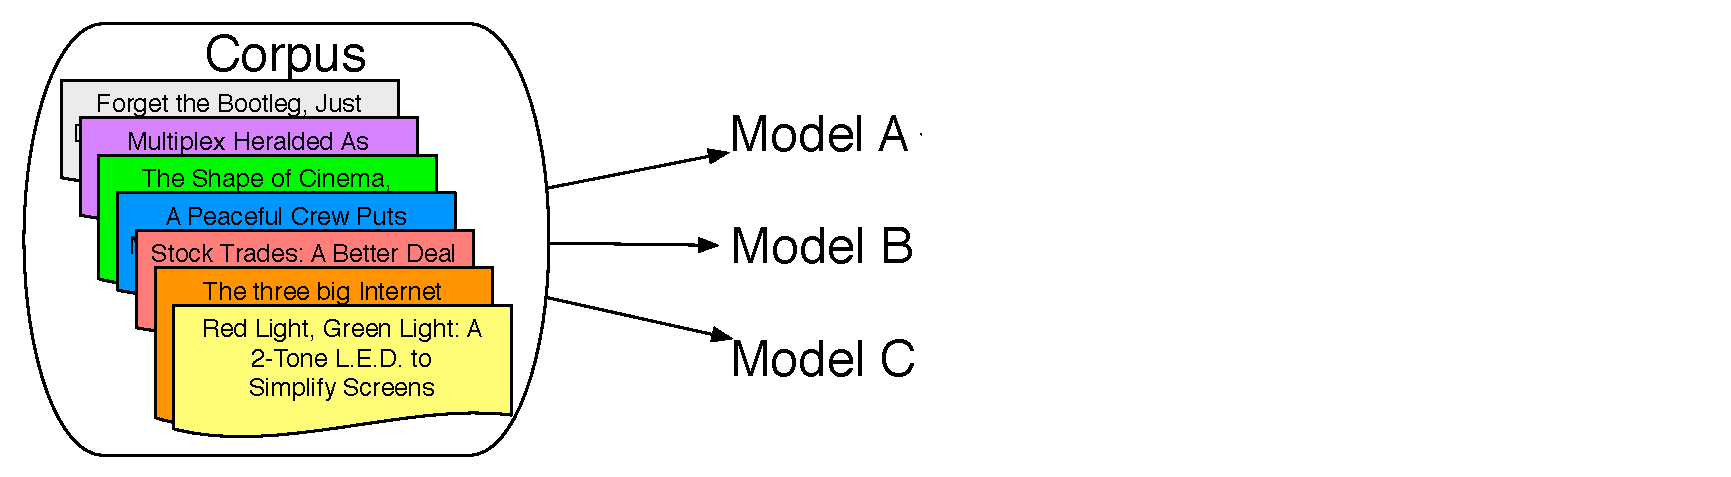
\includegraphics[width=0.9\linewidth]{reading_tea_leaves/figures/heldout_1} }
\only<1>{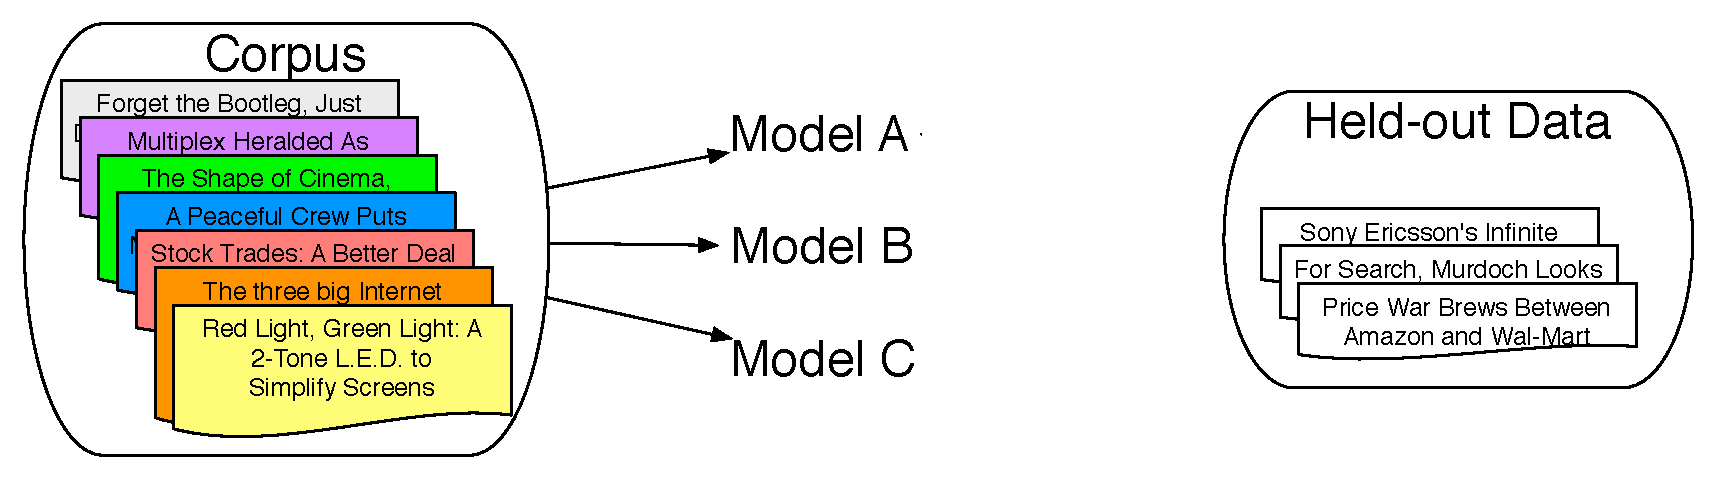
\includegraphics[width=\linewidth]{reading_tea_leaves/figures/heldout_2} }
%\only<3>{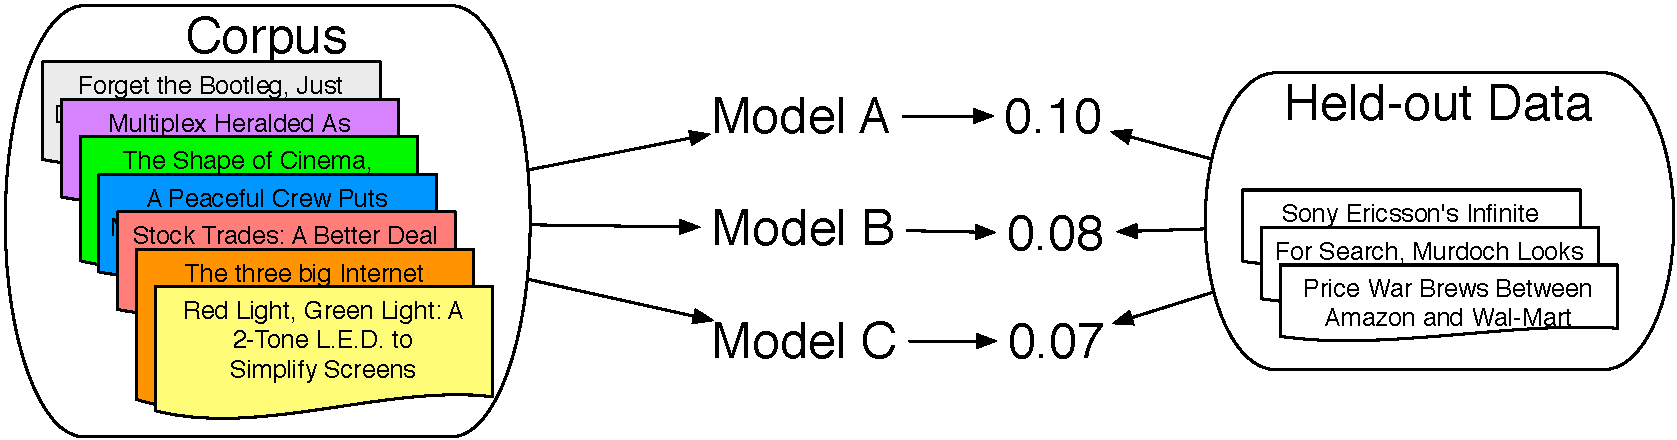
\includegraphics[width=\linewidth]{reading_tea_leaves/figures/heldout_3} }
\only<2>{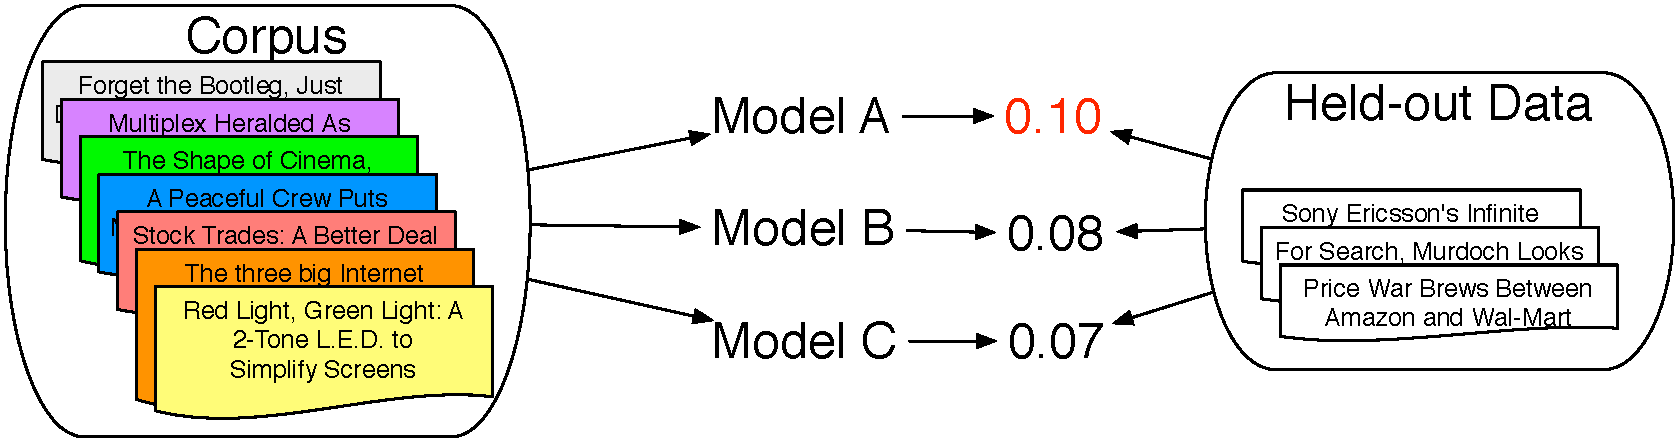
\includegraphics[width=\linewidth]{reading_tea_leaves/figures/heldout_4}  \\
	\large Measures predictive power (likelihood / perplexity), not what the topics are}
\end{center}
}

\frame{
\frametitle{Qualitative Evaluation of the Latent Space}

\begin{center}
\only<1>{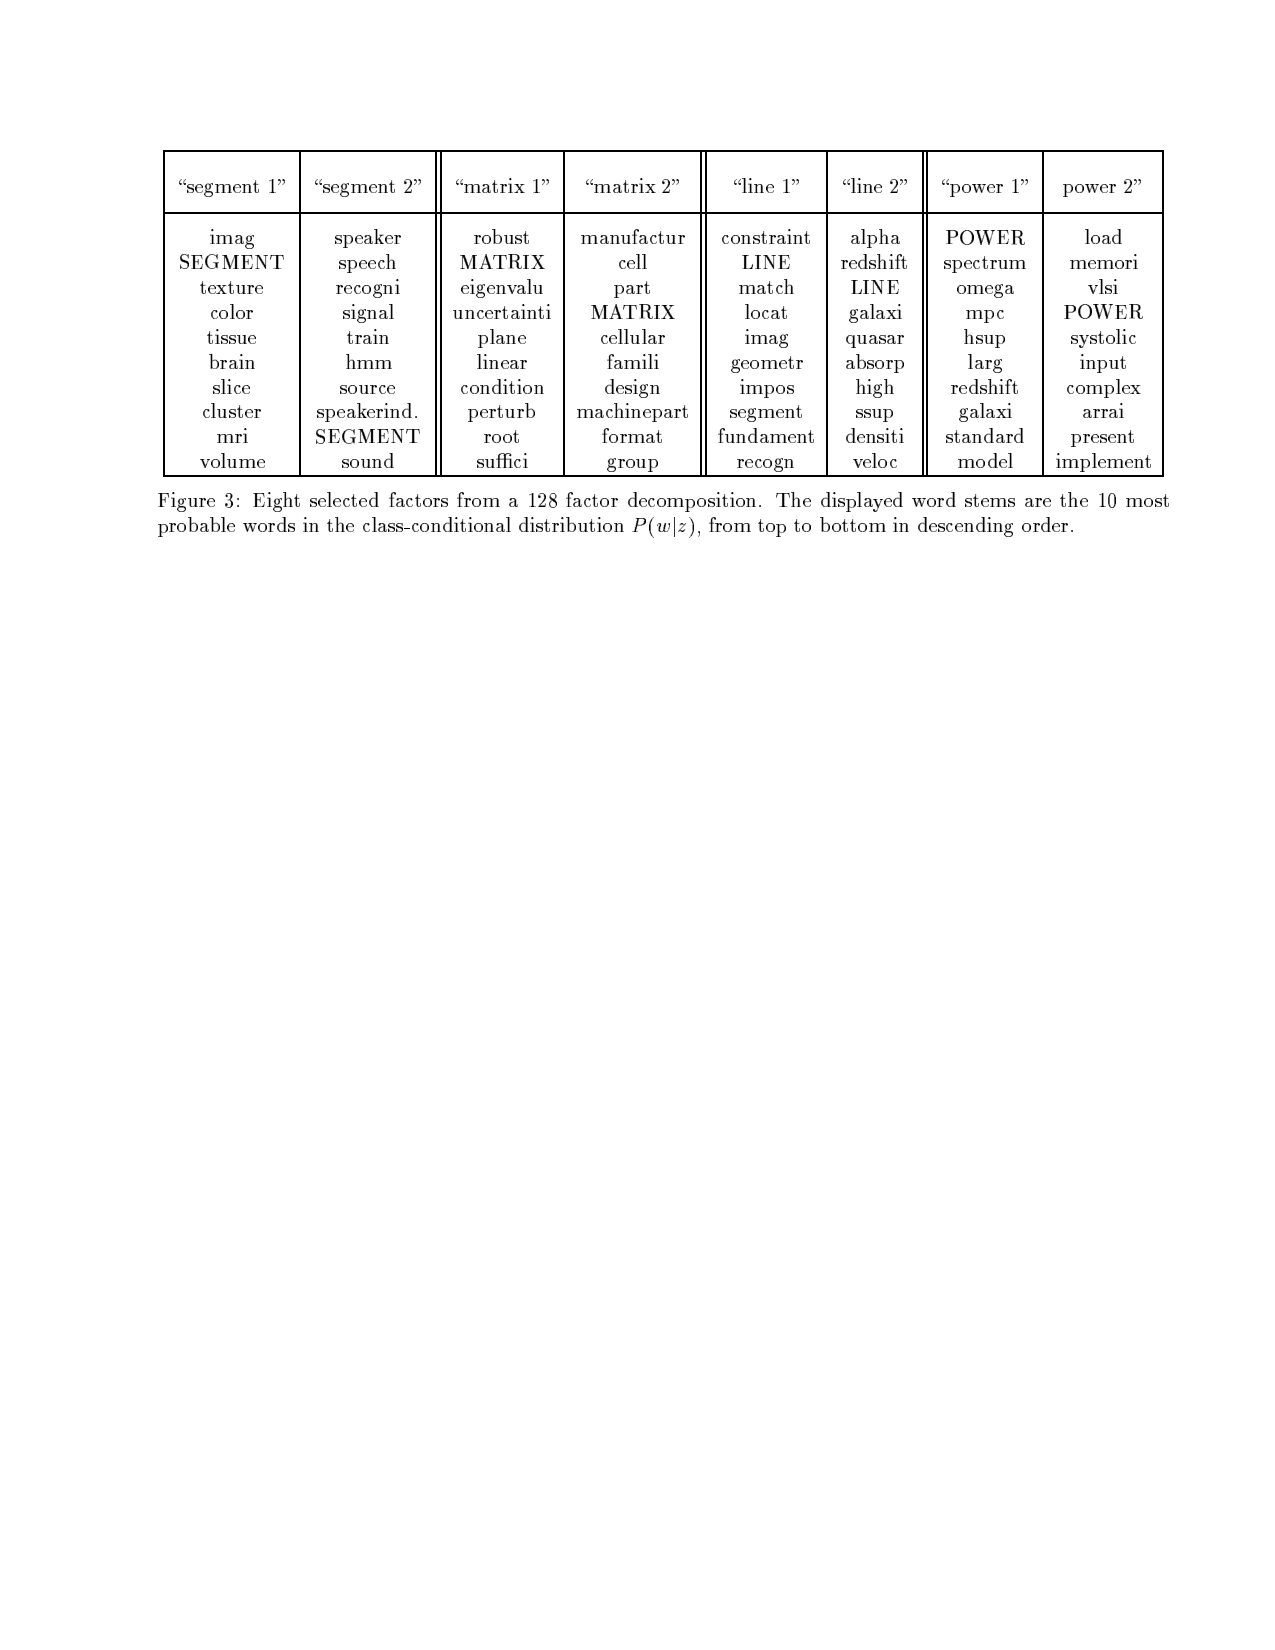
\includegraphics[width=0.9\linewidth]{reading_tea_leaves/topics_from_papers/1} \\ \cite{hofmann-99} }
\only<2>{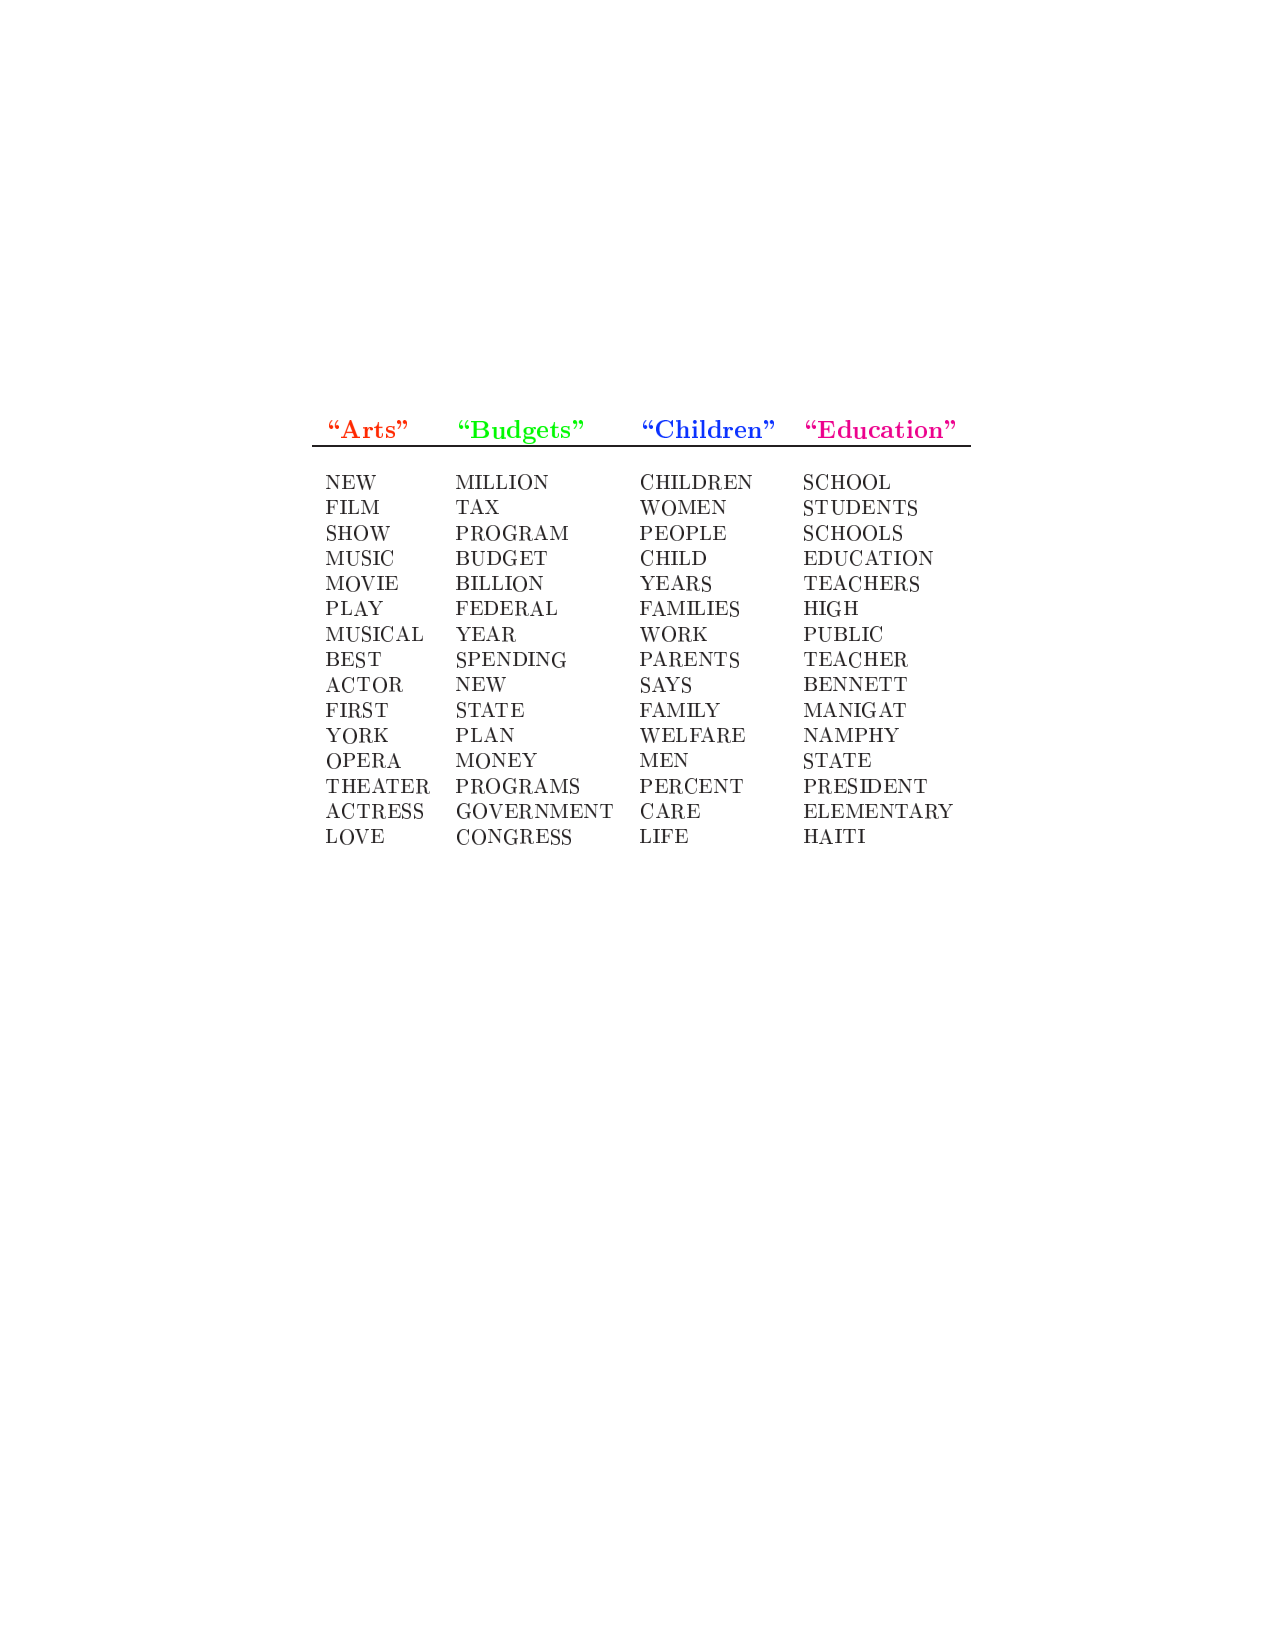
\includegraphics[width=0.7\linewidth]{reading_tea_leaves/topics_from_papers/2} \\ \cite{blei-03} }
\only<3>{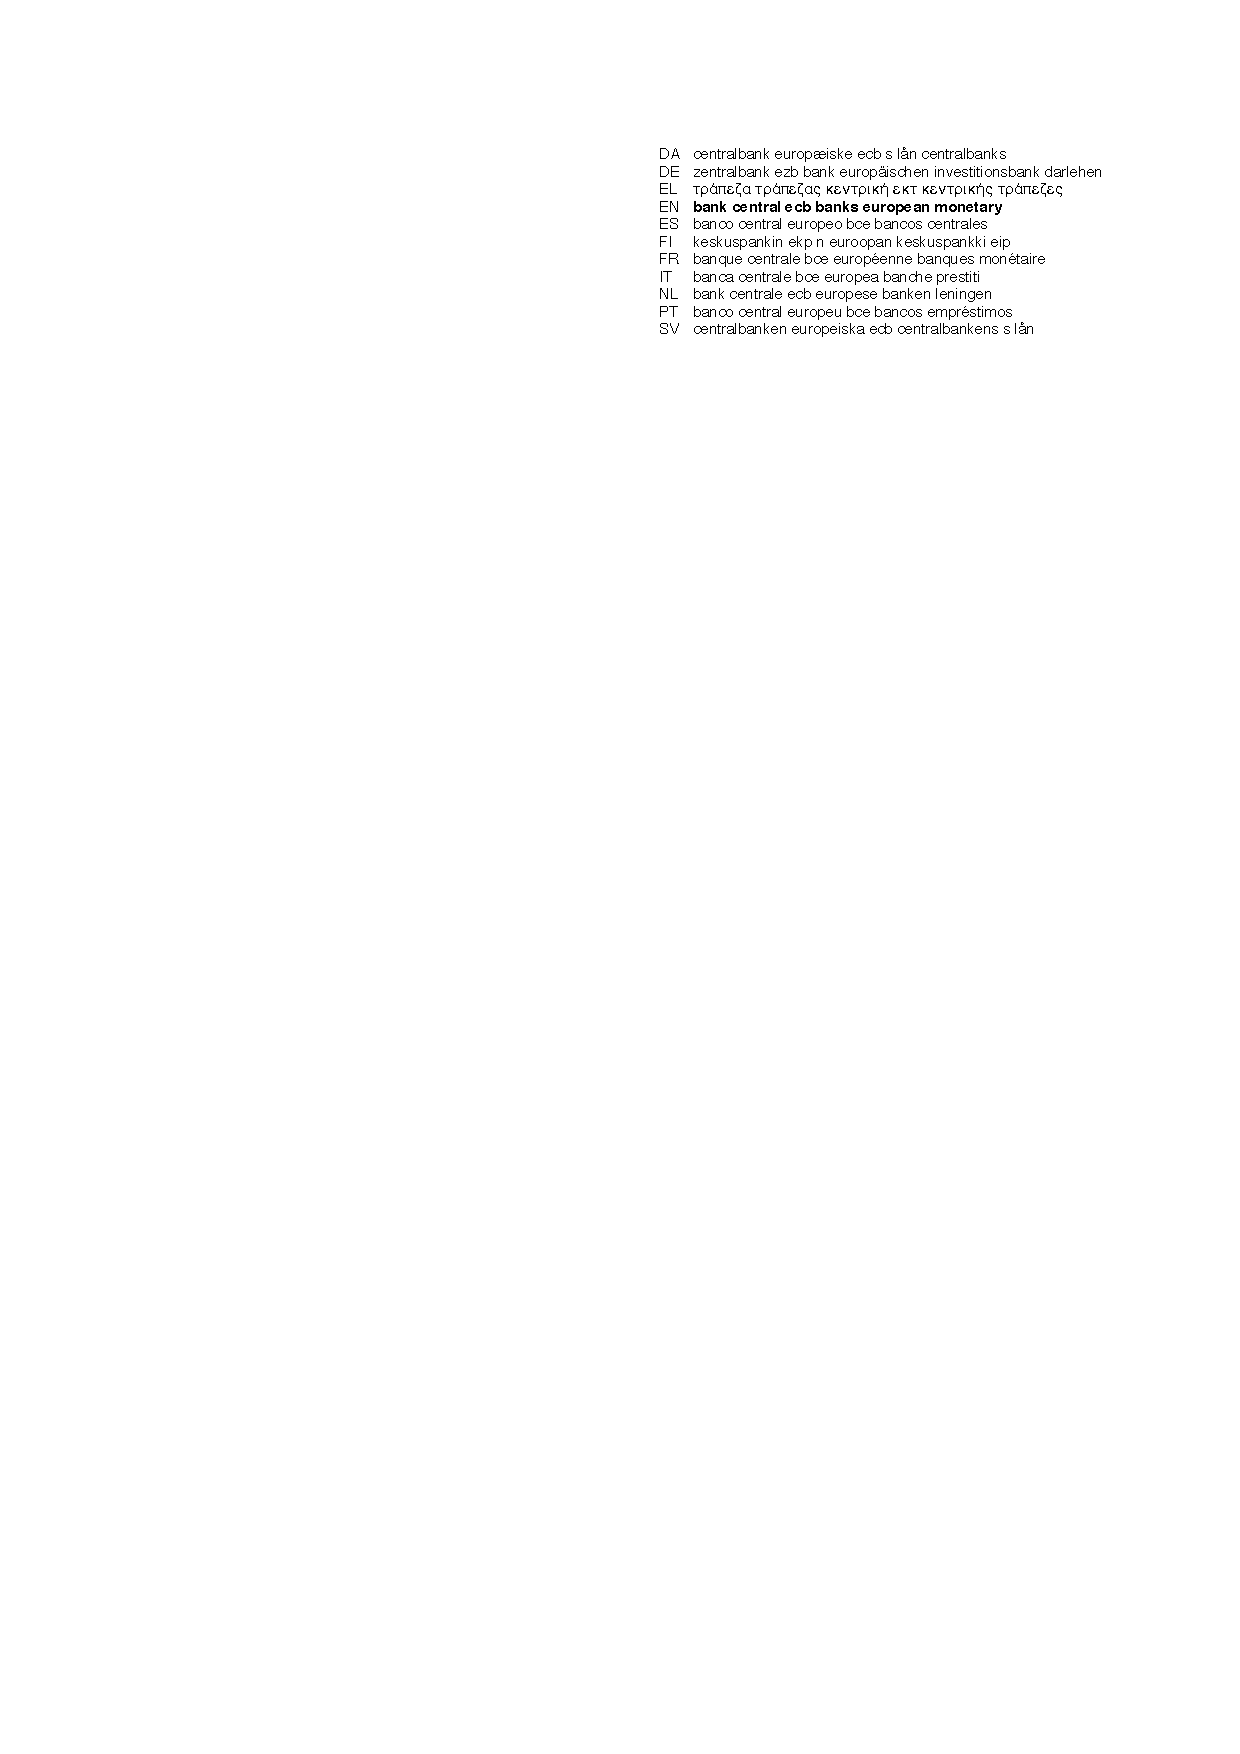
\includegraphics[width=0.7\linewidth]{reading_tea_leaves/topics_from_papers/3} \\ \cite{mimno-09} }
\only<4>{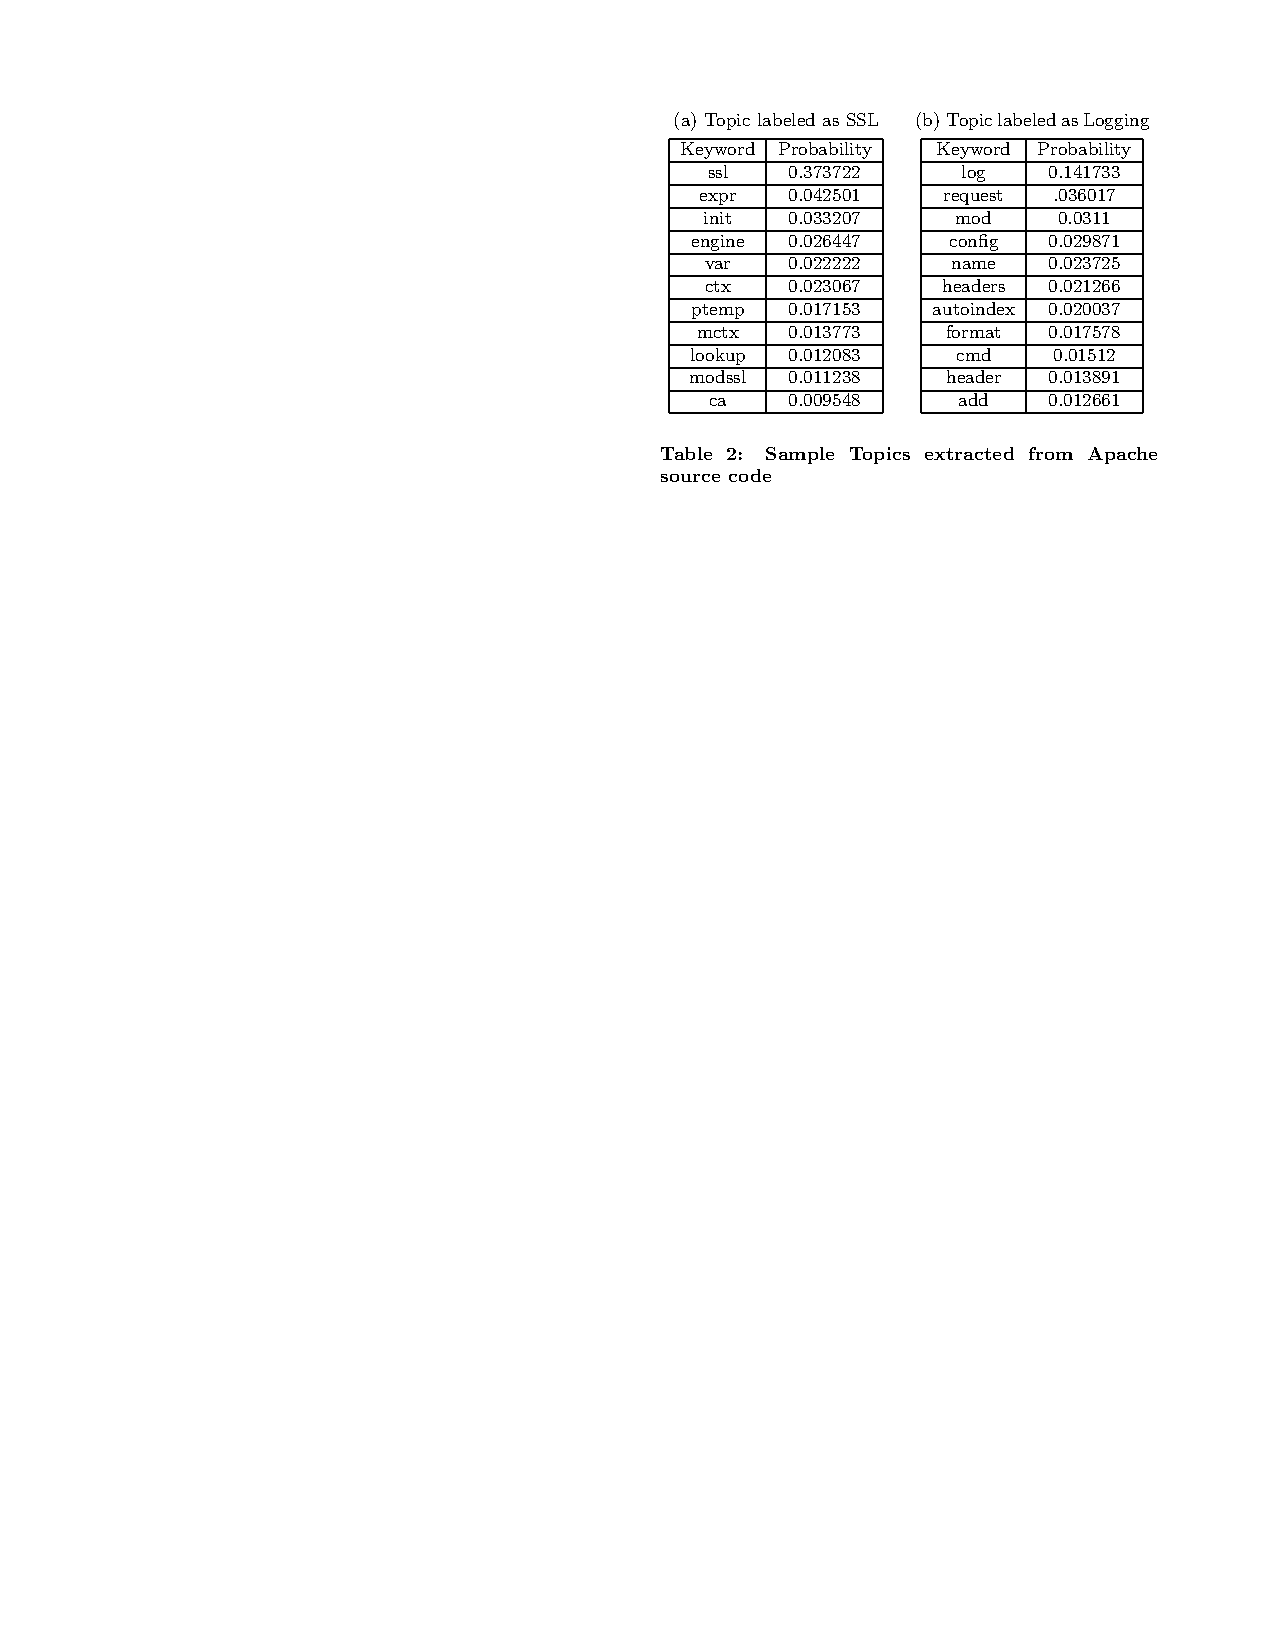
\includegraphics[width=0.7\linewidth]{reading_tea_leaves/topics_from_papers/4} \\ \cite{maskeri-08} }
\only<5>{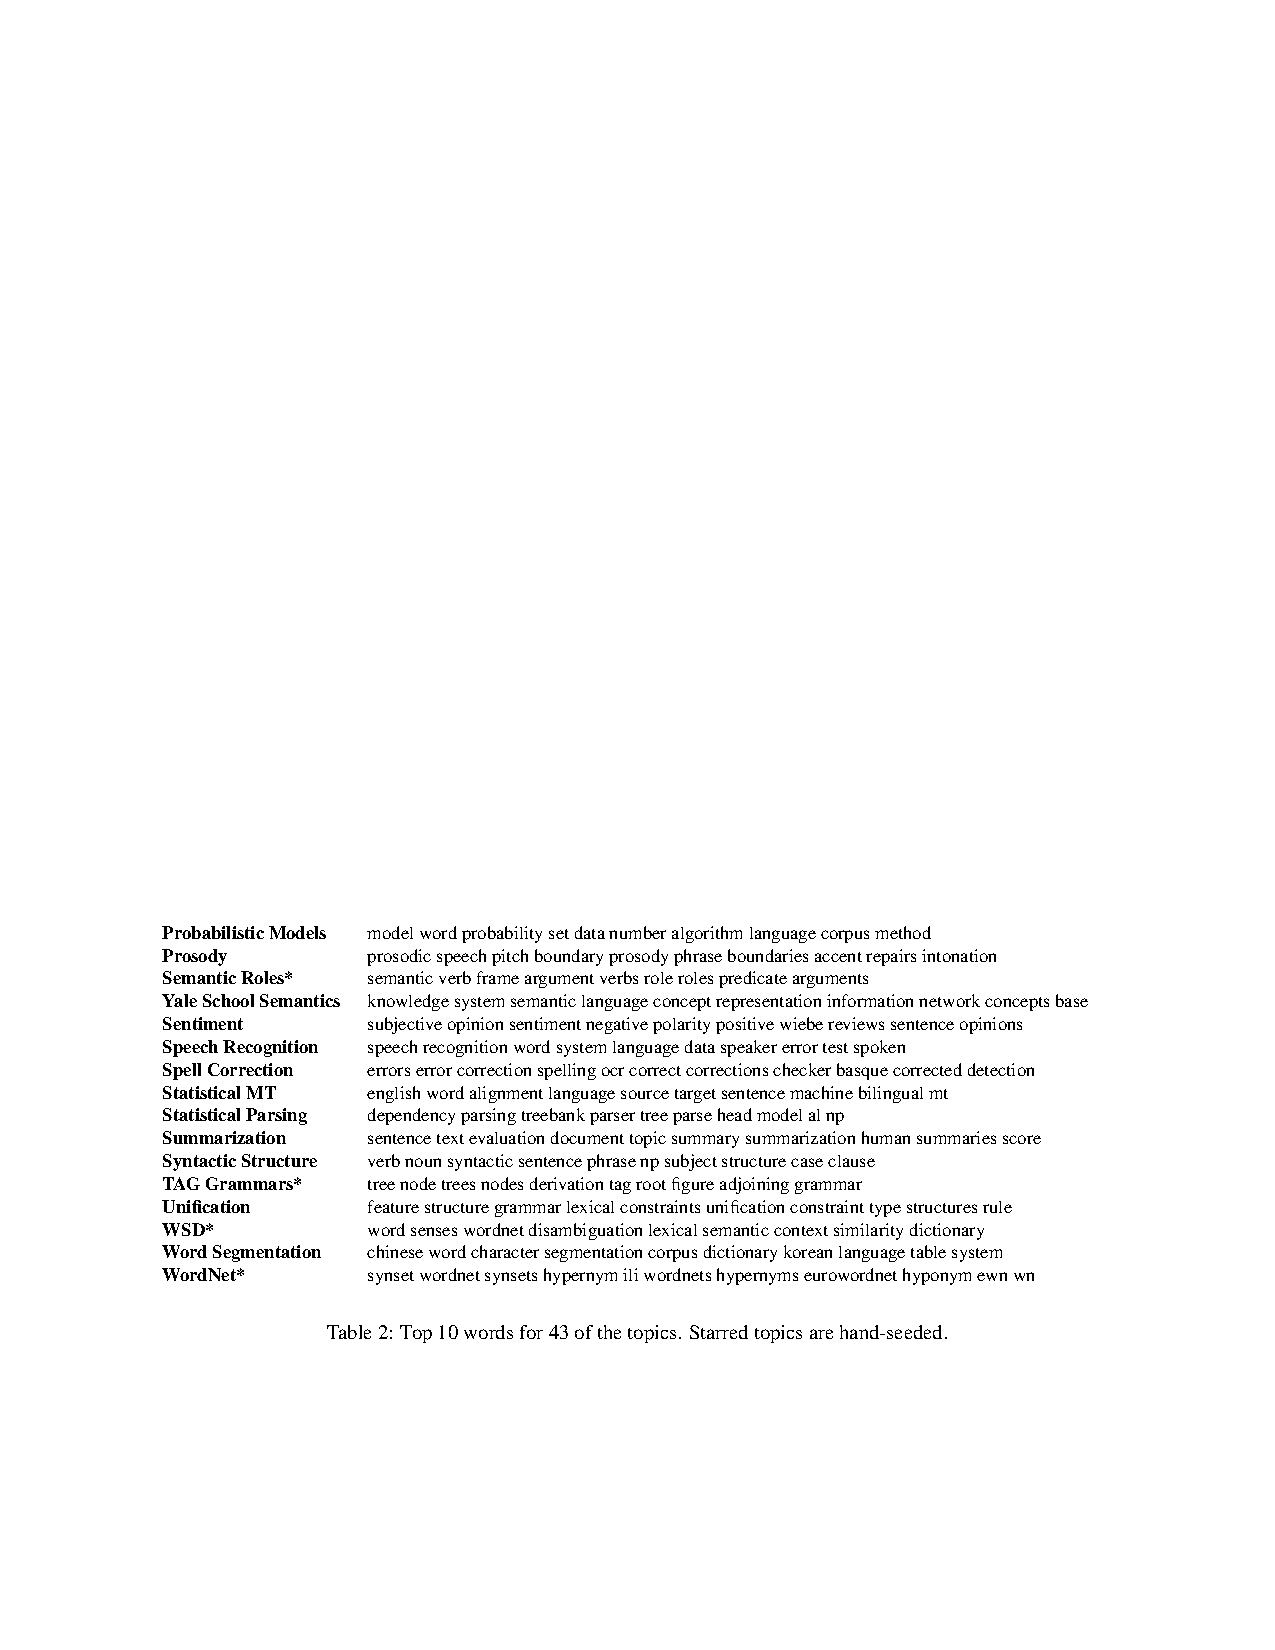
\includegraphics[width=0.9\linewidth]{reading_tea_leaves/topics_from_papers/5} \\ \cite{hall-08} }
\end{center}
}

\frame{
\begin{center}
  \only<1>{
\includegraphics[width=0.8\linewidth]{reading_tea_leaves/topics_from_papers/rexa_logo} \\
    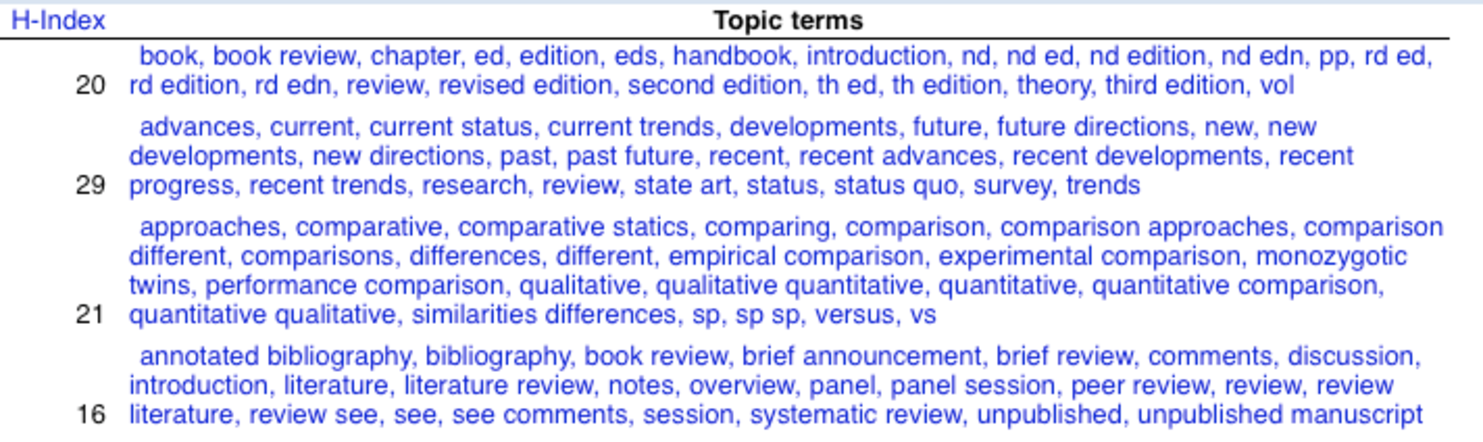
\includegraphics[width=0.8\linewidth]{reading_tea_leaves/topics_from_papers/rexa_topic} \\
    Topics are shown to users during web search.}
  \only<2> {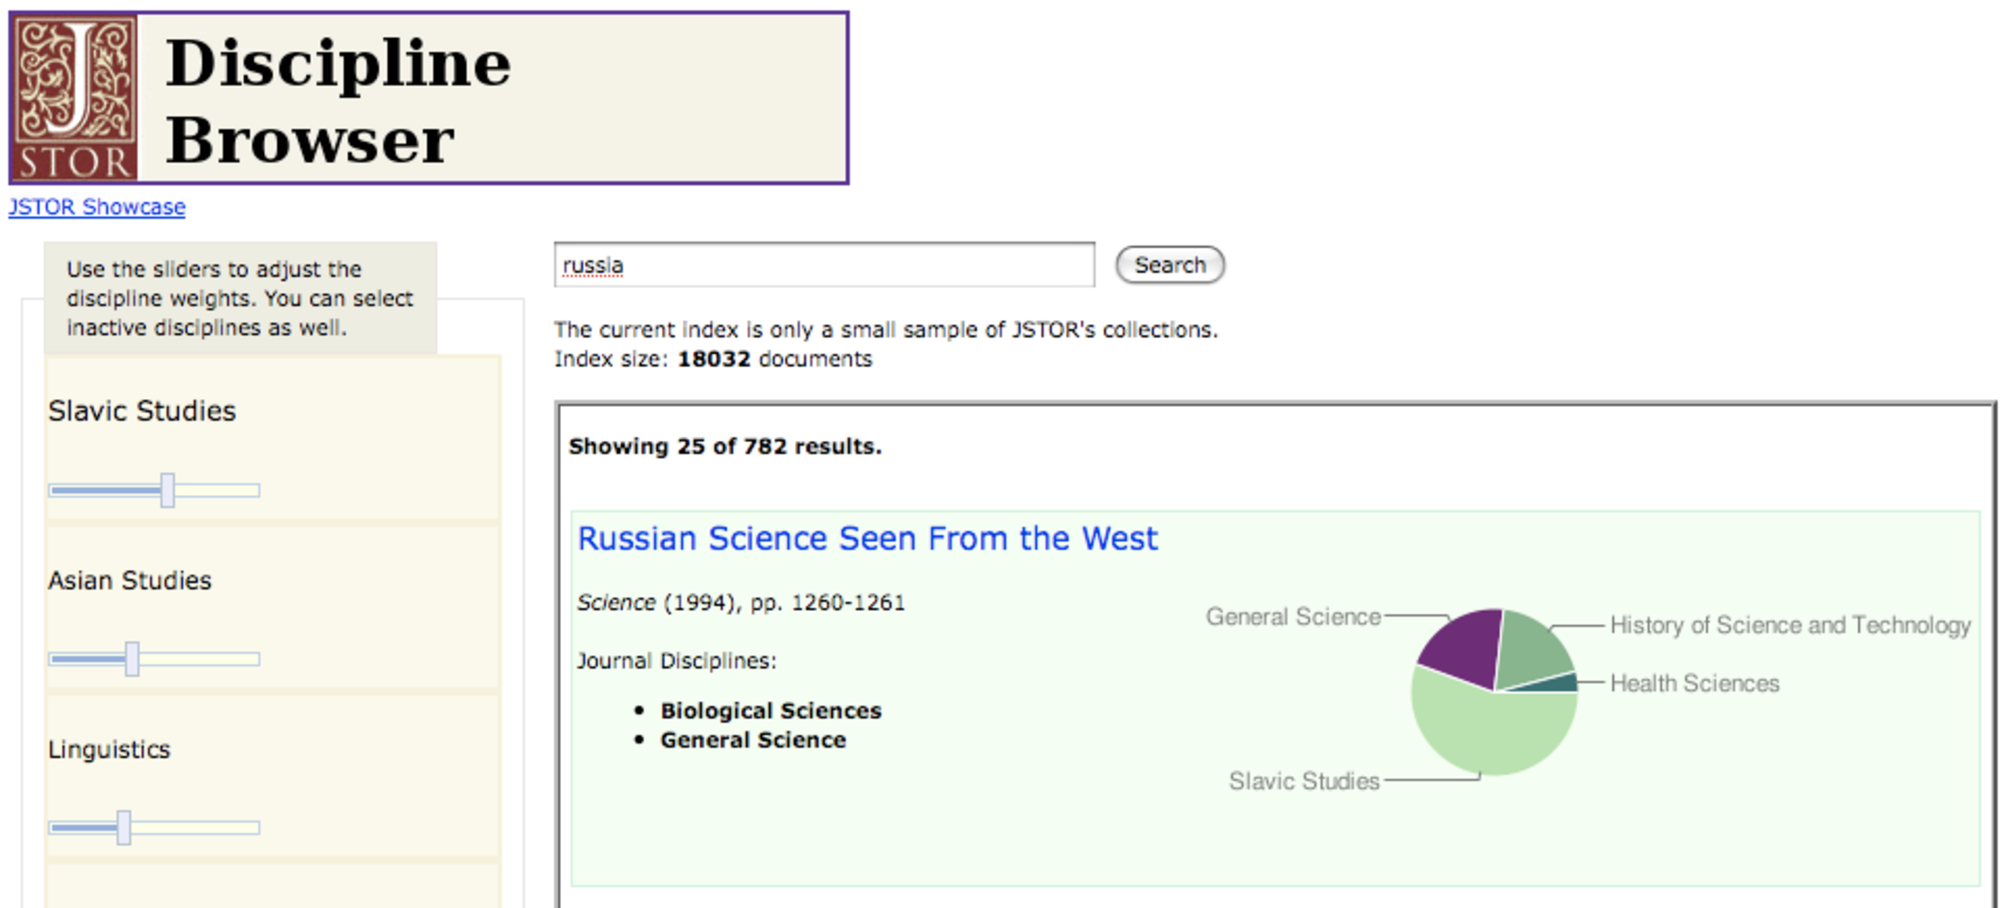
\includegraphics[width=0.9\linewidth]{reading_tea_leaves/topics_from_papers/jstor} \\
    Users can refine queries through topics.}

\end{center}
}

\frame{
\frametitle{Key Points}

\begin{enumerate}
  \item ``Reading Tea Leaves'' alternative: measuring {\bf interpretability}
  \item Direct, quantitative human evaluation of latent space
  \item Testing interpretability on different models and corpora
  \item Disconnect with likelihood
\end{enumerate}
\pause
\begin{columns}
\column{.85\linewidth}
\begin{flushright}
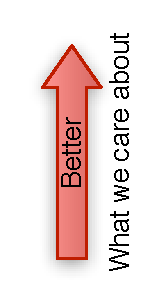
\includegraphics[scale=\graphscale]{reading_tea_leaves/tasks/care_about}
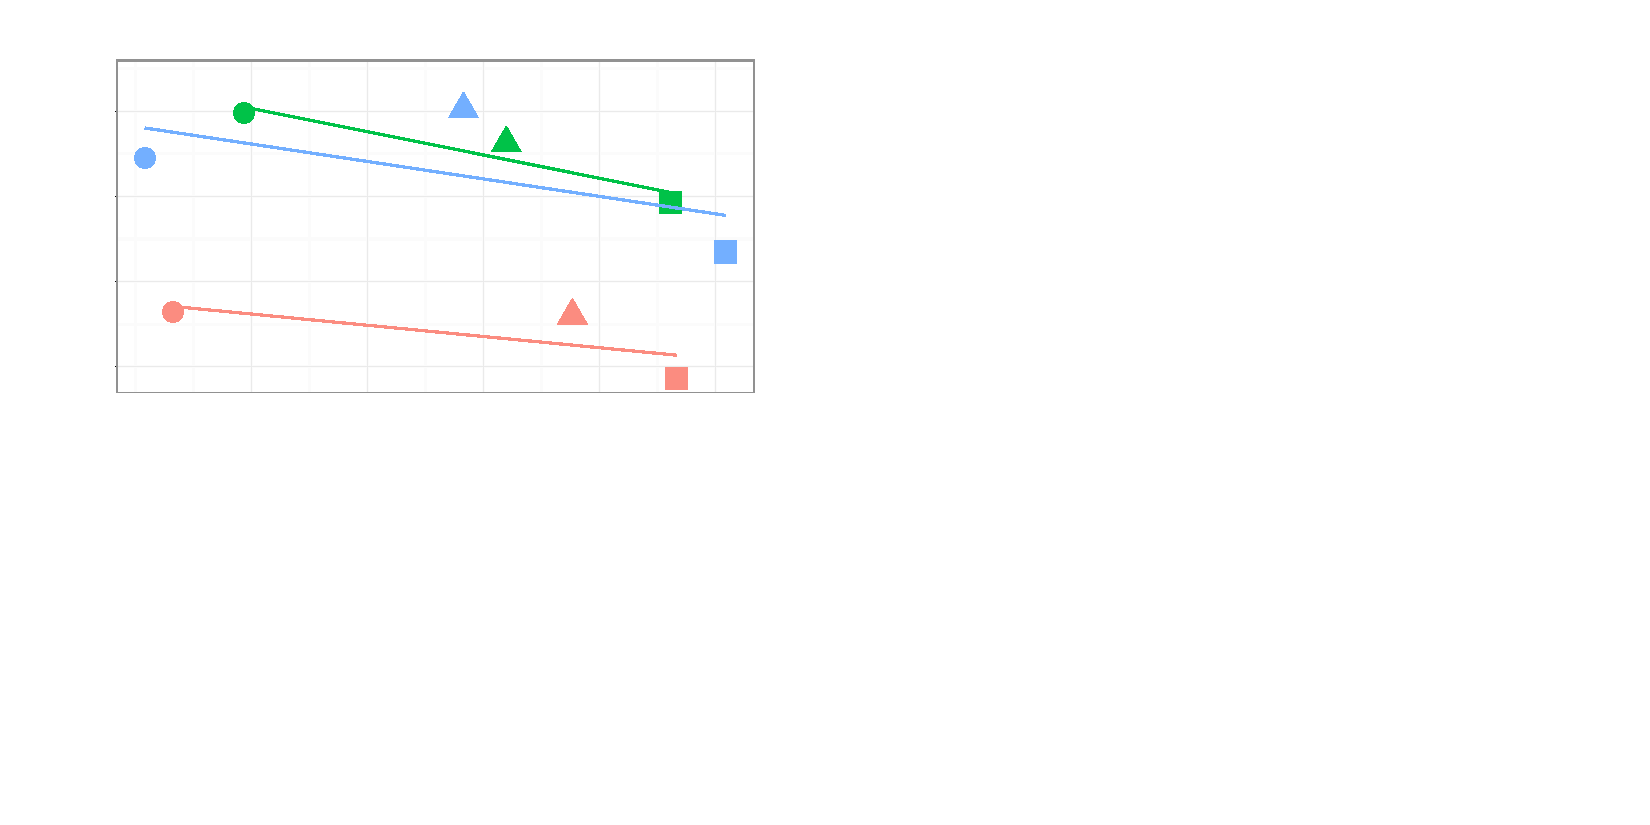
\includegraphics[scale=\graphscale]{reading_tea_leaves/tasks/nyt_mp} \\
\end{flushright}
\column{.15\linewidth}
\end{columns}
\vspace{-.8cm}
\begin{center}
  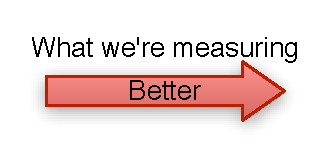
\includegraphics[scale=\graphscale]{reading_tea_leaves/tasks/measuring} \\
\end{center}
}

\frame{
  \frametitle{Evaluating Topic Interpretability}

  \begin{itemize}
   \item Interpretability is a human judgment
    \item We will ask people directly
    \item Experiment Goals
      \begin{itemize}
        \item Quick
        \item Fun
        \item Consistent
      \end{itemize}
      \pause
      \item We turn to Amazon Mechanical Turk
        \iflong
       \item Two tasks: Word Intrusion and Topic Intrusion
         \else
         \item Primary task: Word Intrusion
         \fi

  \end{itemize}
}

\frame{
\frametitle{Data from the Cloud}
\begin{columns}[c]


\column{0.45\linewidth}

\begin{block}{Then}
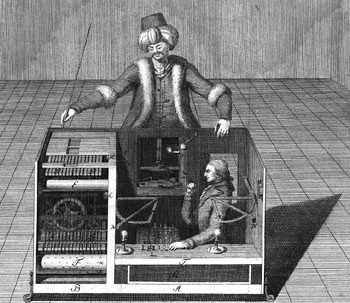
\includegraphics[width=0.95\linewidth]{evocation/figures/mechanical_turk_old}
\end{block}


\column{0.45\linewidth}

\begin{block}{Now}
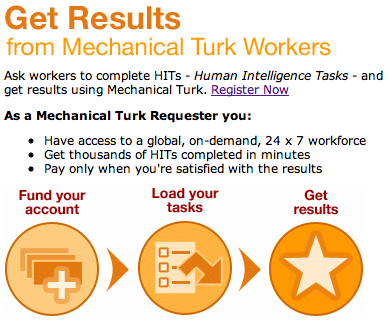
\includegraphics[width=0.95\linewidth]{evocation/figures/mechanical_turk_new}
\end{block}

\end{columns}
}


\frame{
  \iflong
  \frametitle{Task One: Word Intrusion}
  \else
  \frametitle{Word Intrusion}
  \fi

  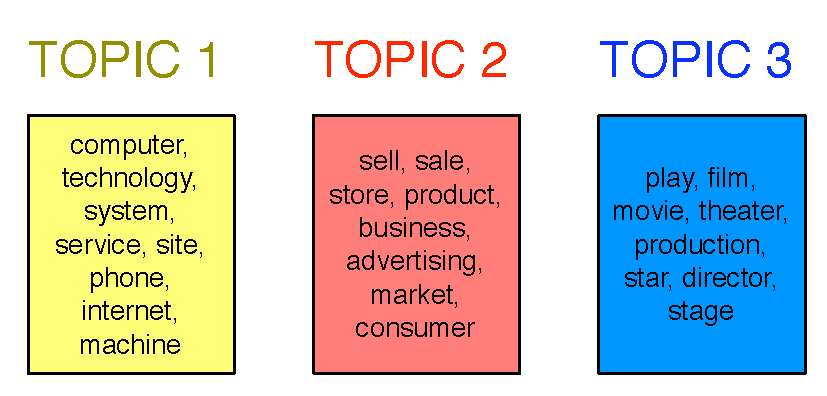
\includegraphics[width=\linewidth]{reading_tea_leaves/figures/nyt_topics_wide}
}


\frame{
  \iflong
  \frametitle{Task One: Word Intrusion}
  \else
  \frametitle{Word Intrusion}
  \fi

  \begin{enumerate}
    \item Take the highest probability words from a topic

      \begin{block}{Original Topic}
        dog, cat, horse, pig, cow
      \end{block}
\pause
    \item Take a high-probability word from another topic and add it
      \begin{block}{Topic with Intruder}
        dog, cat, \alert<2->{apple}, horse, pig, cow
      \end{block}
\pause
     \item We ask users to find the word that doesn't belong
  \end{enumerate}
\begin{block}{Hypothesis}
If the topics are interpretable, users will consistently choose true intruder
\end{block}
}

\frame{
  \iflong
  \frametitle{Task One: Word Intrusion}
  \else
  \frametitle{Word Intrusion}
  \fi
\begin{center}
\only<1>{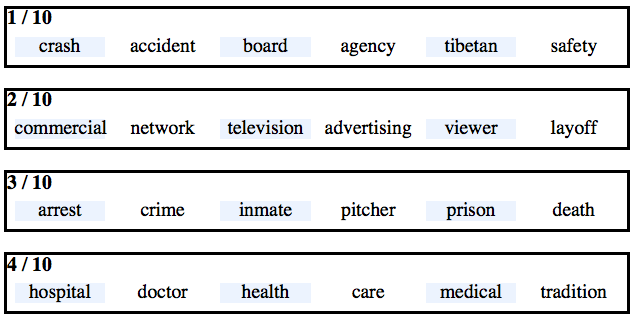
\includegraphics[width=\linewidth]{reading_tea_leaves/tasks/word1}  }
\only<2>{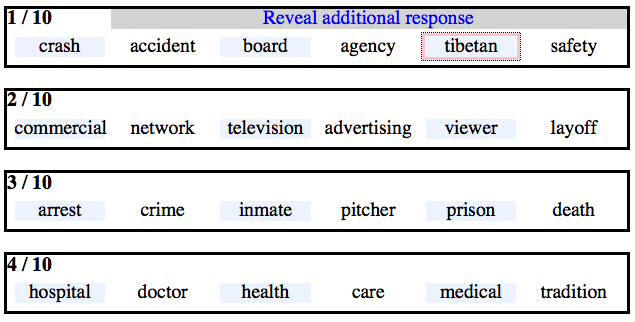
\includegraphics[width=\linewidth]{reading_tea_leaves/tasks/word2}  }
\pause
  \begin{itemize}
    \item Order of words was shuffled
    \item Which intruder was selected varied
    \item Model precision: percentage of users who clicked on intruder
  \end{itemize}

\end{center}
}

\iflong


\frame{
   \frametitle{Task Two: Topic Intrusion}
	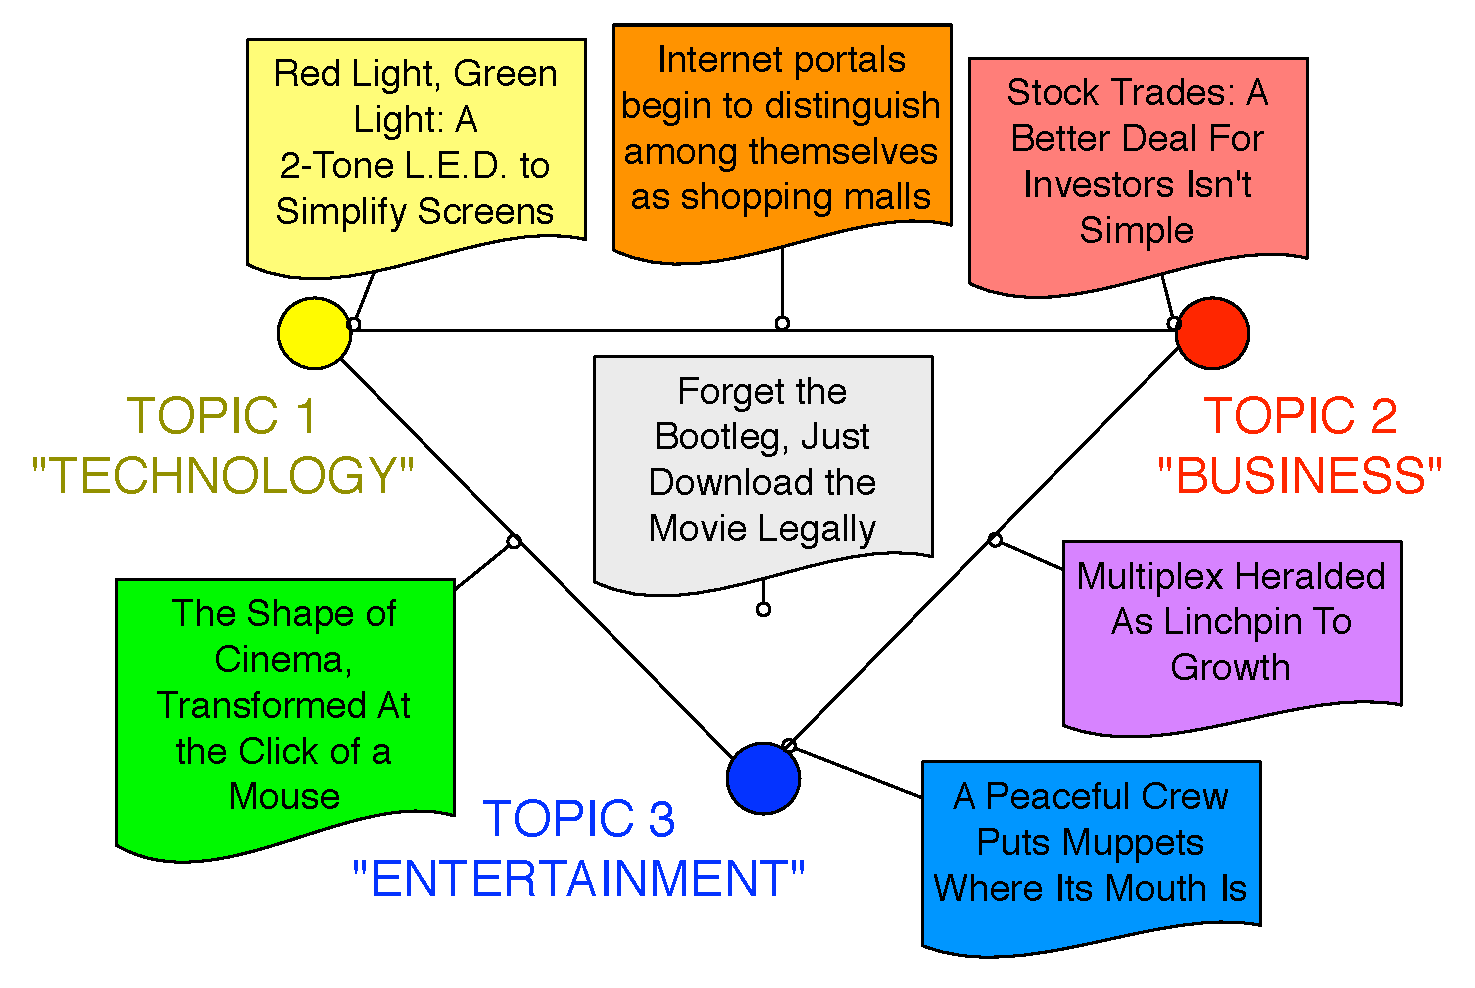
\includegraphics[width=\linewidth]{reading_tea_leaves/figures/nyt_documents}
}

\frame{
   \frametitle{Task Two: Topic Intrusion}
  \begin{enumerate}
    \item Display document title and first 500 characters to users
    \item Show the three topics with highest probability and one topic chosen randomly
    \item Have the user click on the the set of words that is out of place
\end{enumerate}
\pause
\begin{block}{Hypothesis}
If the association of topics to a document is interpretable, users will consistently choose true intruding topic
\end{block}
}

\frame{
  \frametitle{Task Two: Topic Intrusion}
\begin{center}
\only<1>{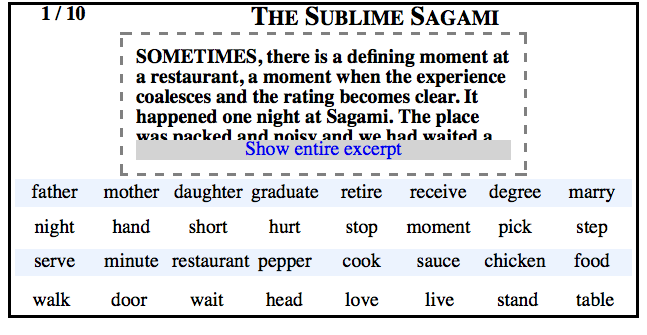
\includegraphics[width=\linewidth]{reading_tea_leaves/tasks/topic2}  }
\only<2>{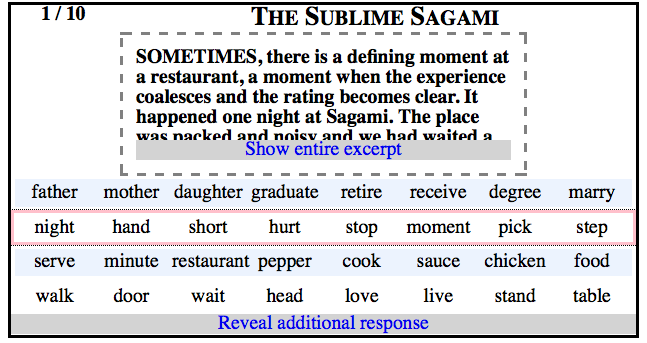
\includegraphics[width=\linewidth]{reading_tea_leaves/tasks/topic3}  }
\end{center}
}

\frame{
   \frametitle{Task Two: Topic Intrusion}
\only<1>{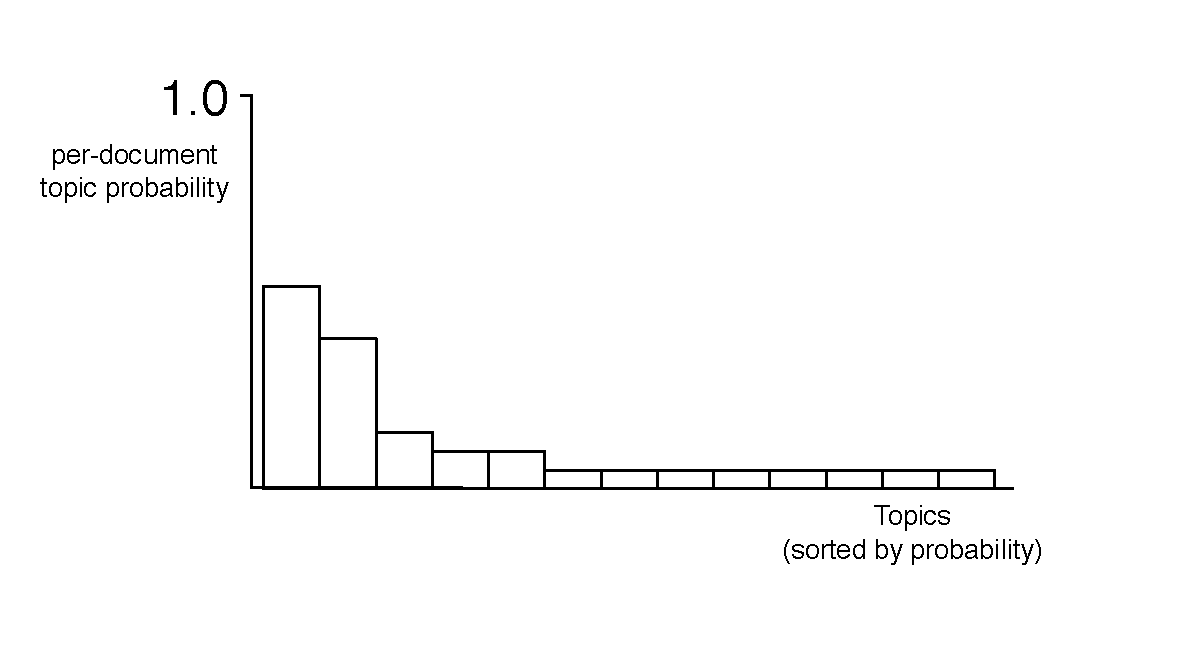
\includegraphics[width=\linewidth]{reading_tea_leaves/figures/tlo_1}  }
\only<2>{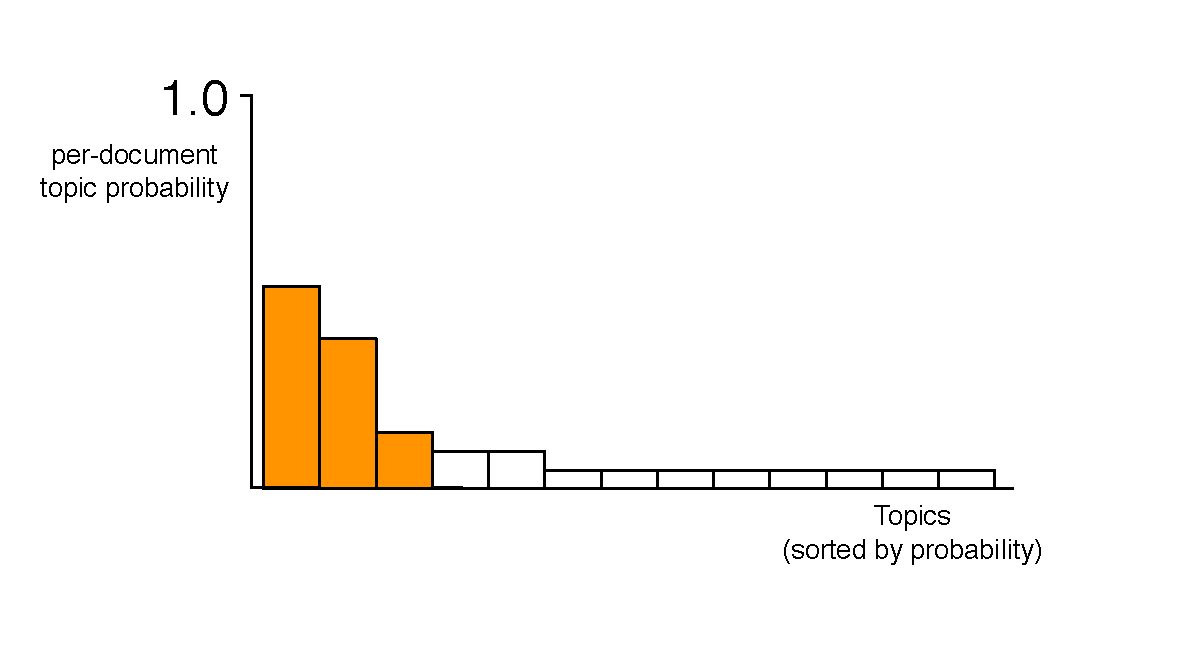
\includegraphics[width=\linewidth]{reading_tea_leaves/figures/tlo_2}  }
\only<3>{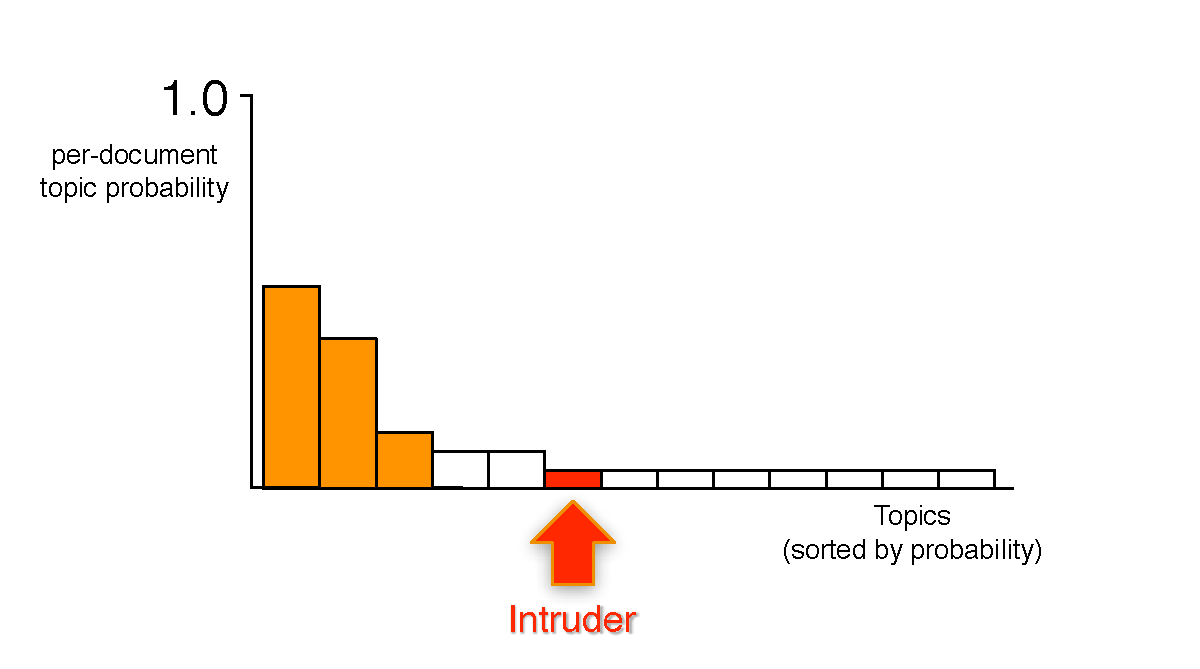
\includegraphics[width=\linewidth]{reading_tea_leaves/figures/tlo_3}  }
\only<4>{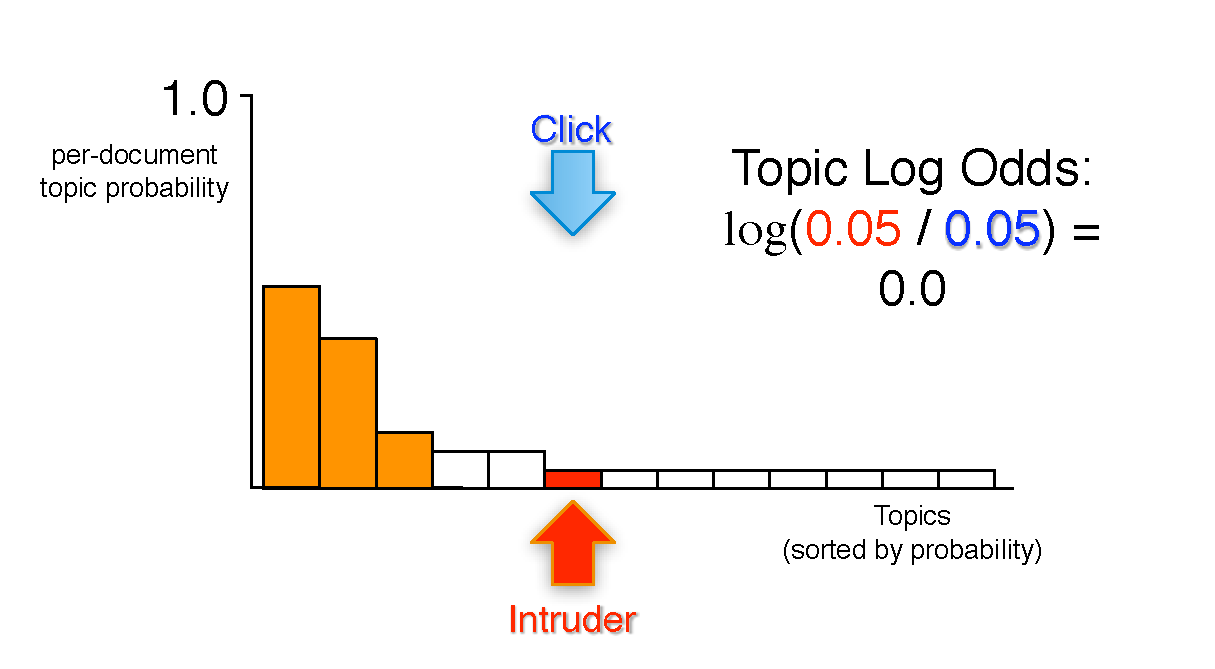
\includegraphics[width=\linewidth]{reading_tea_leaves/figures/tlo_4}  }
\only<5>{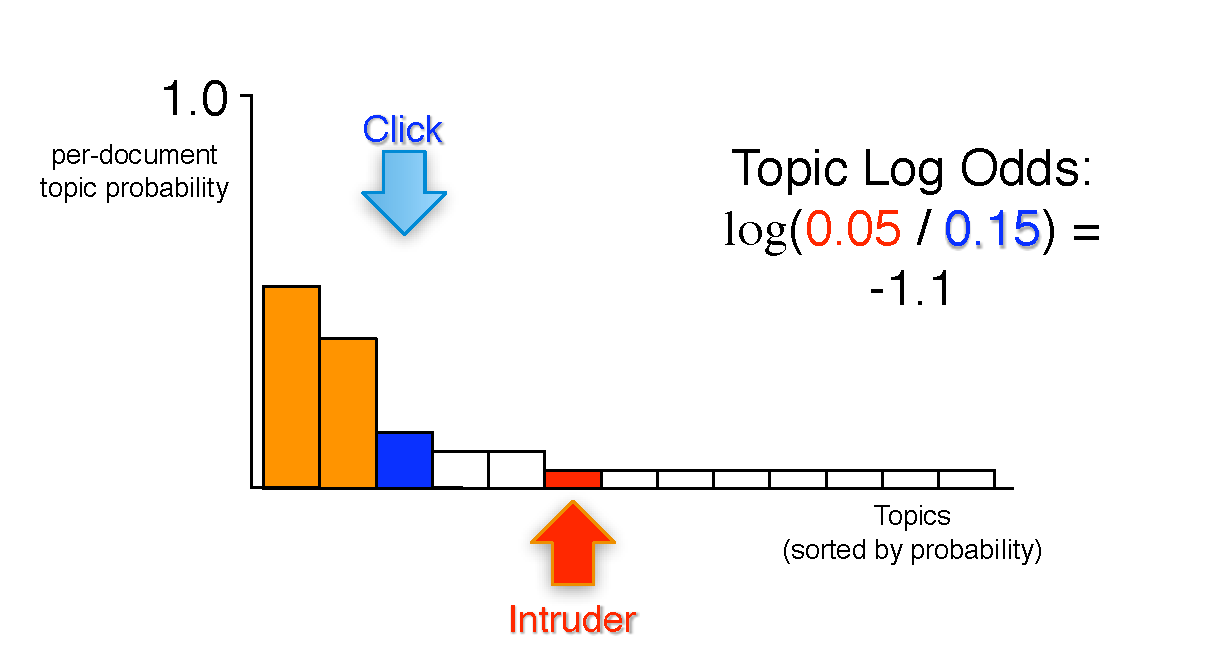
\includegraphics[width=\linewidth]{reading_tea_leaves/figures/tlo_5}  }
\only<6>{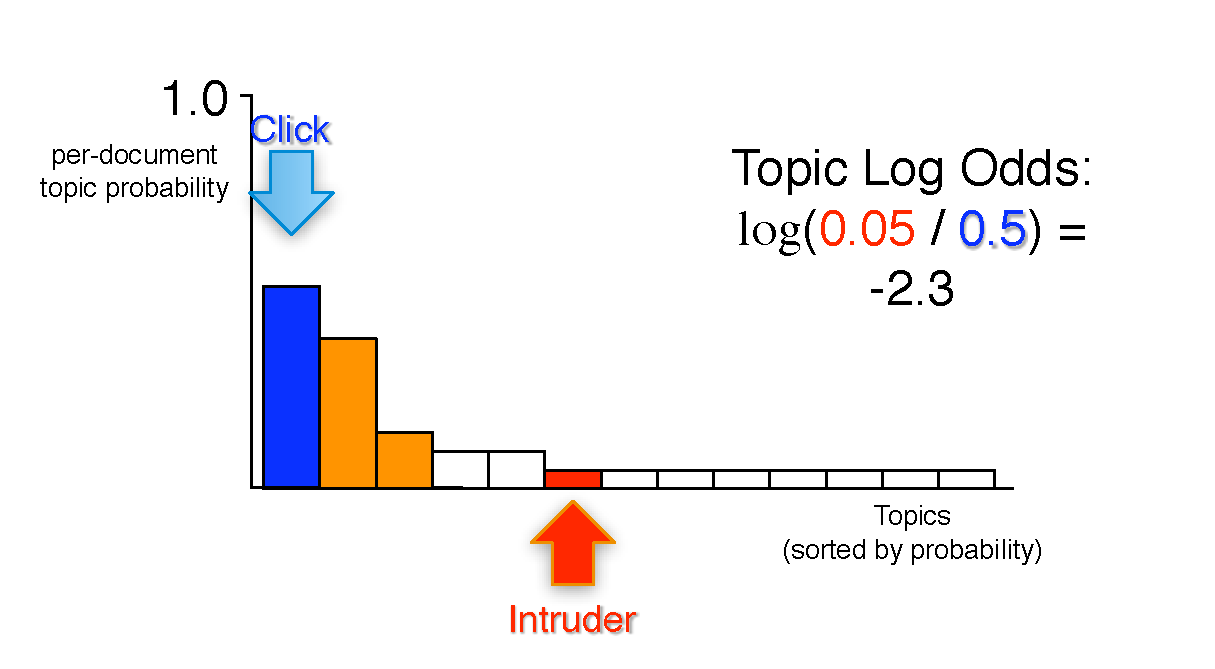
\includegraphics[width=\linewidth]{reading_tea_leaves/figures/tlo_6}  }
}
\else


\fi

\frame{
\frametitle{Three Topic Models}
Different assumptions lead to different topic models
\begin{itemize}
  \item Free parameter: probabilistic latent semantic indexing (pLSI)~\cite{hofmann-99}
  \item Dirichlet: latent Dirichlet allocation (LDA)~\cite{blei-03}
  \item Normal with covariance: correlated topic model (CTM)~\cite{blei-06}
\end{itemize}
}

\frame{
\frametitle{Corpora}

\begin{columns}
\column{.45\linewidth}
\center{\includegraphics[width=0.9\linewidth]{reading_tea_leaves/corpora/nyt} }
\column{.45\linewidth}
\center{ \includegraphics[width=0.5\linewidth]{reading_tea_leaves/corpora/wikipedia-logo} }
\end{columns}

\begin{columns}
\column{.45\linewidth}
\begin{itemize}
  \item 8477 articles
  \item 8269 types
  \item 1M tokens
\end{itemize}

\column{.45\linewidth}
\begin{itemize}
  \item Sample of 10000 articles
  \item 15273 types
  \item 3M tokens
\end{itemize}
\end{columns}

\pause

\begin{block}{Corpora properties}
\begin{itemize}
  \item Well structured (should begin with summary paragraph)
  \item Real-world
  \item Many different themes
\end{itemize}
\end{block}
}

\frame{
\frametitle{Experiments}
\begin{enumerate}
 \item Fit pLSI, LDA, and CTM to both corpora
 \item Each model had 50, 100, or 150 topics
 \item 50 topics from each condition presented to 8 workers
\iflong
 \item 100 documents form each condition presented to 8 workers
\fi
\end{enumerate}
}

\frame{
\frametitle{Word Intrusion: Which Topics are Interpretable?}
  \begin{block}{New York Times, 50 LDA Topics}
    \begin{center}
      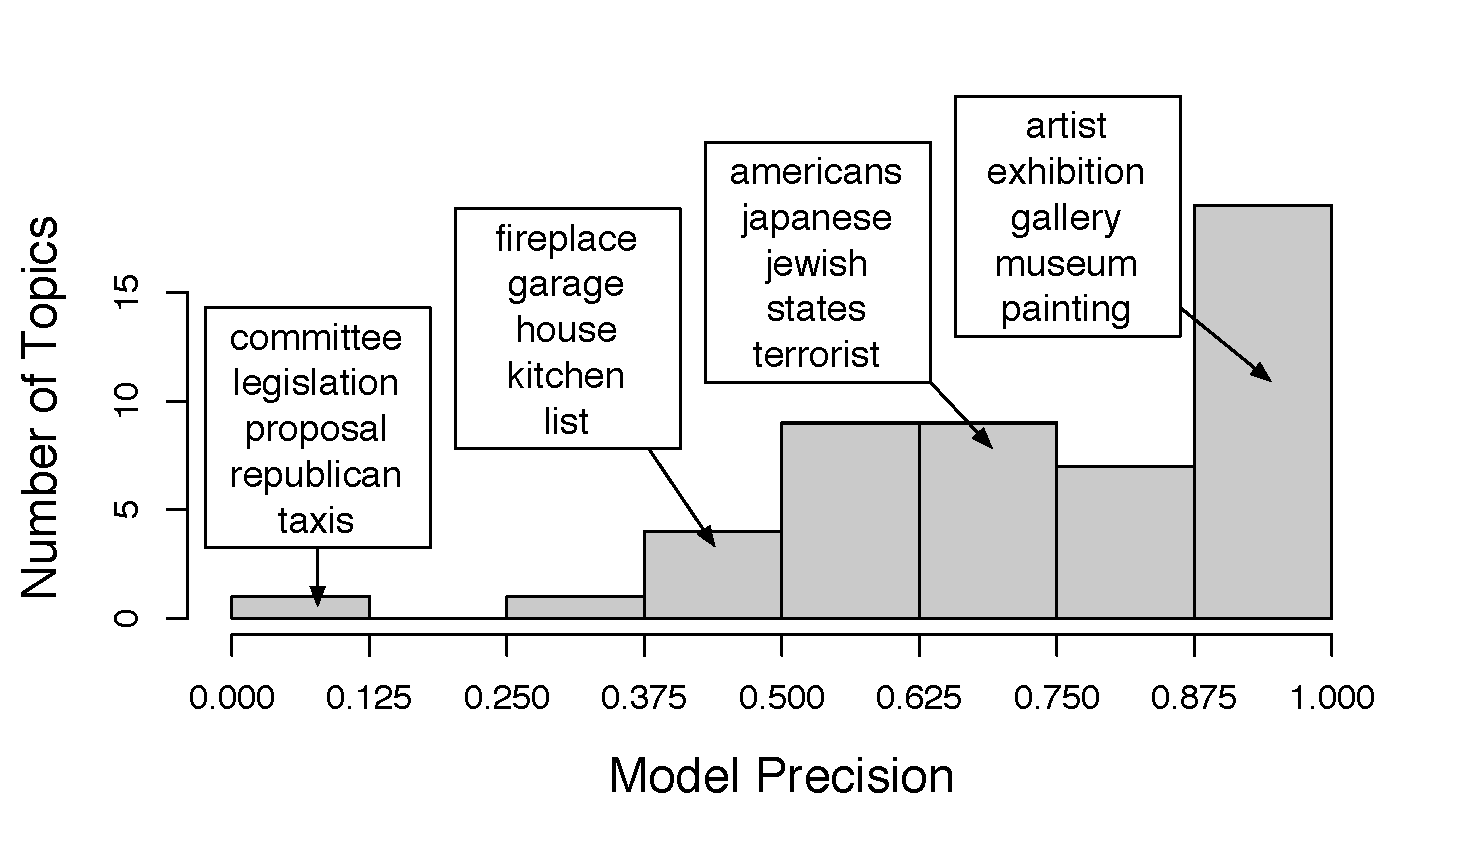
\includegraphics[width=0.8\linewidth]{reading_tea_leaves/figures/topic_precision}
    \end{center}
  \end{block}
  \begin{center}
    Model Precision: percentage of correct intruders found
  \end{center}
}

\iflong

\frame{
\frametitle{Word intrusion: Models with Interpretable Topics}
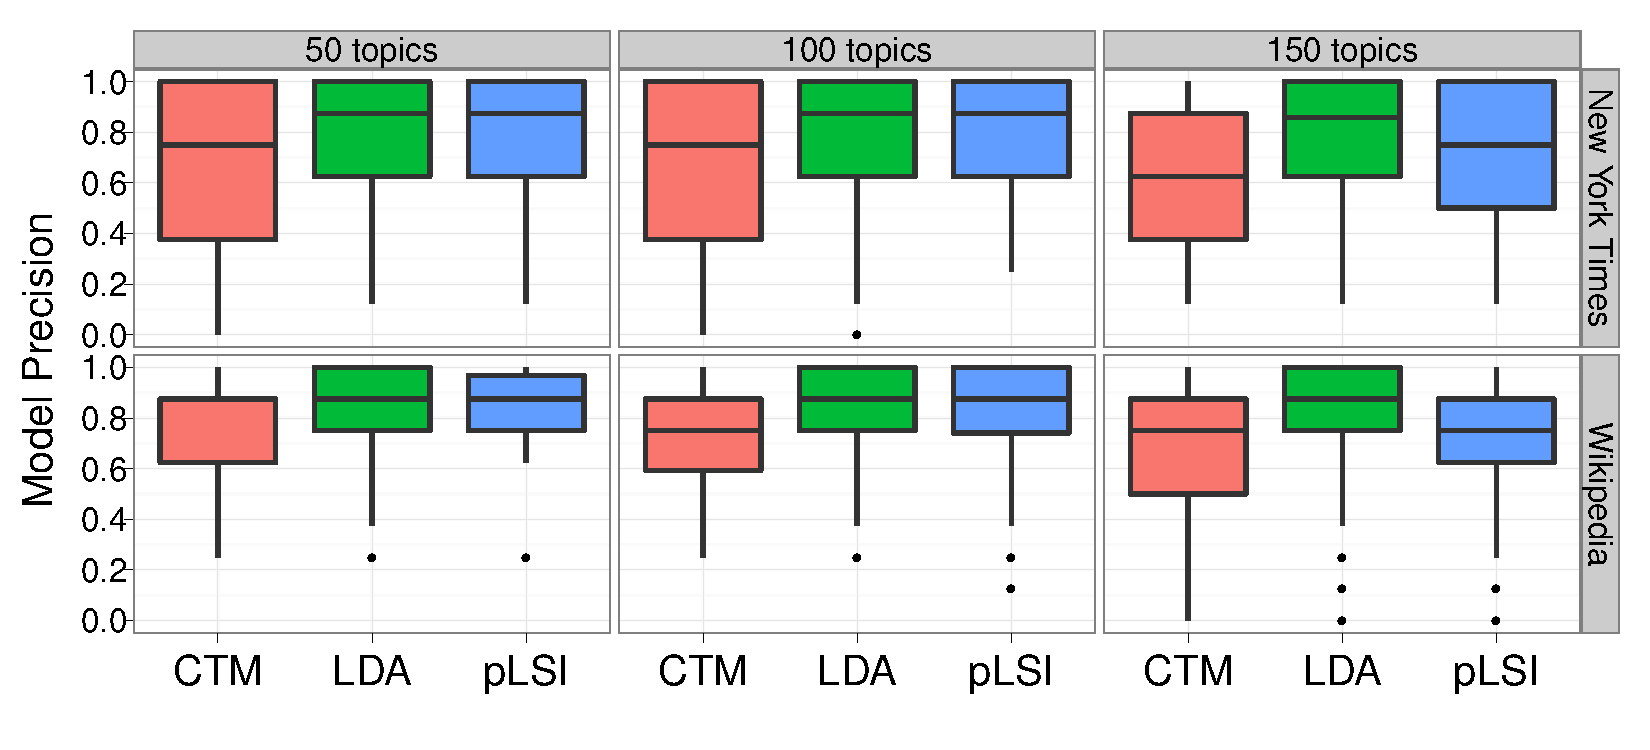
\includegraphics[width=1.0\textwidth]{reading_tea_leaves/tasks/precision}
}

\fi

\iflong

\frame{
  \frametitle{Which documents have clear topic associations?}
  \begin{block}{Wikipedia, 50 LDA Topics}
    \begin{center}
      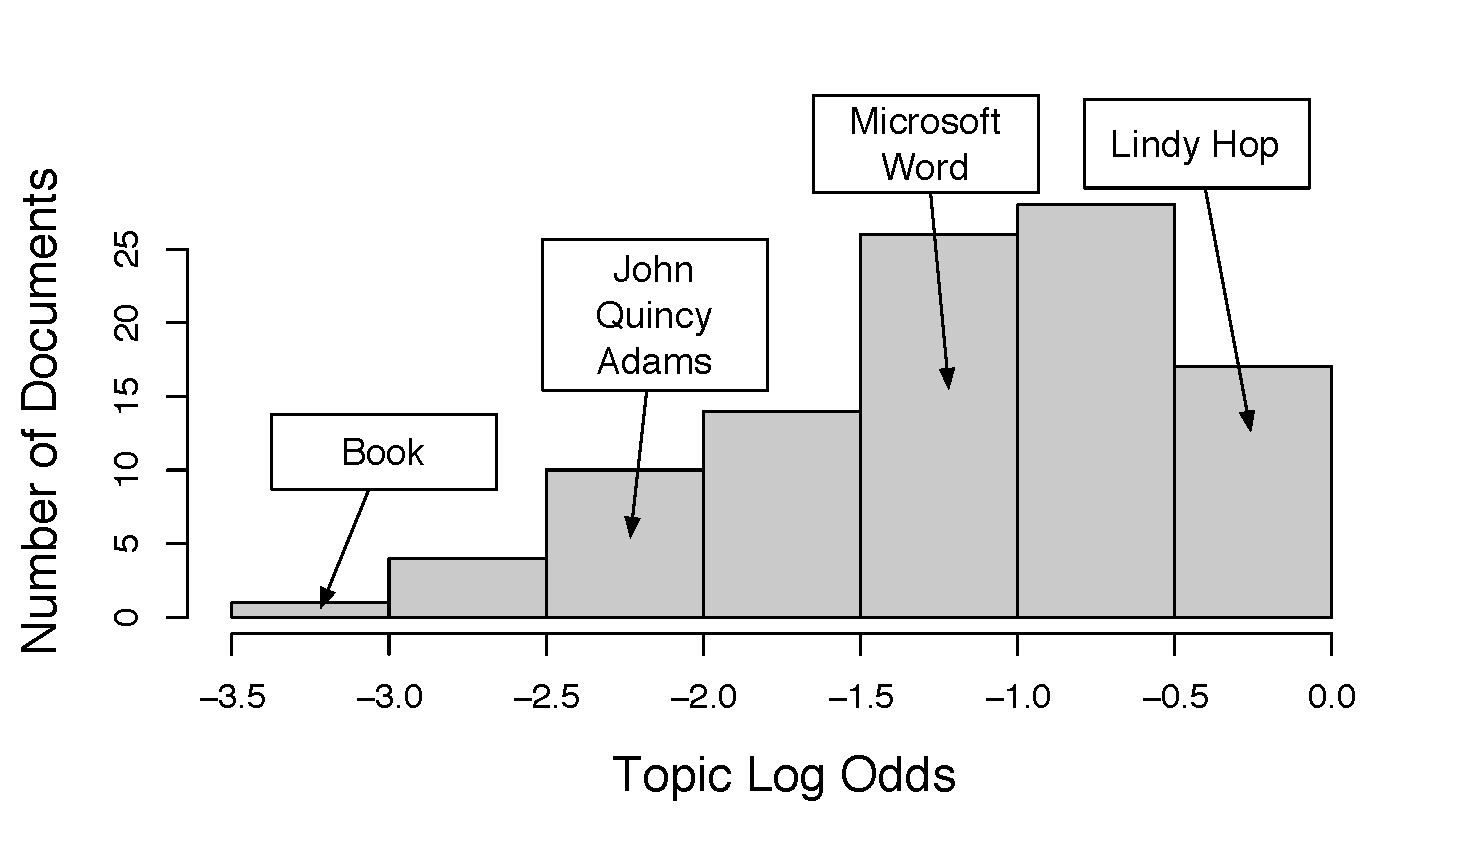
\includegraphics[width=0.8\linewidth]{reading_tea_leaves/figures/document_odds}
    \end{center}
  \end{block}
}


\frame{
\frametitle{Which Models Produce Interpretable Topics}
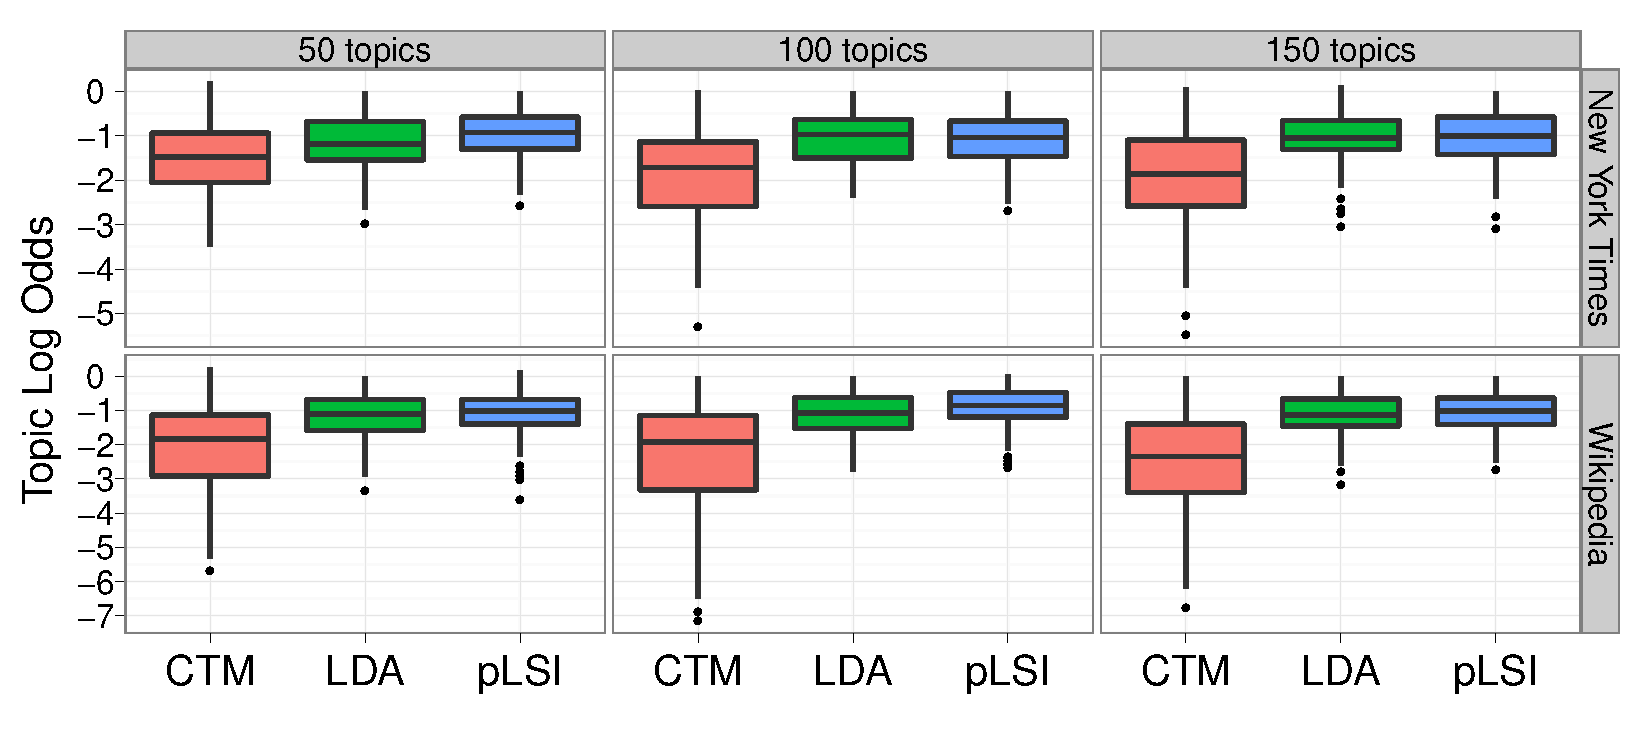
\includegraphics[width=1.0\textwidth]{reading_tea_leaves/tasks/topic_odds}
}

\frame{
  \frametitle{Held-out Likelihood}

\begin{center}

\begin{tabular}{c|c|ccc}
%% \hline
%%  & & \multicolumn{3}{c|}{Model} \\
Corpus & Topics & pLSI & LDA & CTM \\
\hline
\multirow{3}{*}{New York Times}
& 50  & -7.3384 &  \alert<1>{{\bf-7.3214}}  &    -7.3335 \\
& 100  & -7.2834 &  -7.2761 & \alert<1>{{\bf -7.2647}} \\
& 150 & \alert<1>{{\bf -7.2382}} &  -7.2477 & -7.2467  \\
\hline
\multirow{3}{*}{Wikipedia}
& 50  & -7.5378 & \alert<1>{{\bf -7.5257}} & -7.5332 \\
& 100  & -7.4748 & -7.4629 & \alert<1>{{\bf -7.4385}} \\
& 150 & -7.4355 & -7.4266 & \alert<1>{{\bf -7.3872}} \\
\hline
\end{tabular}

\end{center}

}


\fi

\frame{

\frametitle{Interpretability and Likelihood}
\begin{center}
\only<1>{Model Precision on New York Times}
\iflong
\only<2>{Topic Log Odds on Wikipedia}
\fi
\end{center}

\begin{columns}
\column{.85\linewidth}
\begin{flushright}
  \only<1>{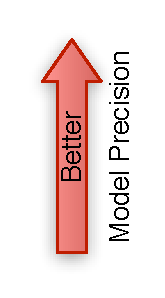
\includegraphics[scale=\graphscale]{reading_tea_leaves/tasks/mp}}
\iflong
  \only<2>{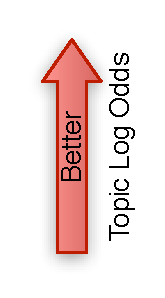
\includegraphics[scale=\graphscale]{reading_tea_leaves/tasks/tlo}}
\fi
  \only<1>{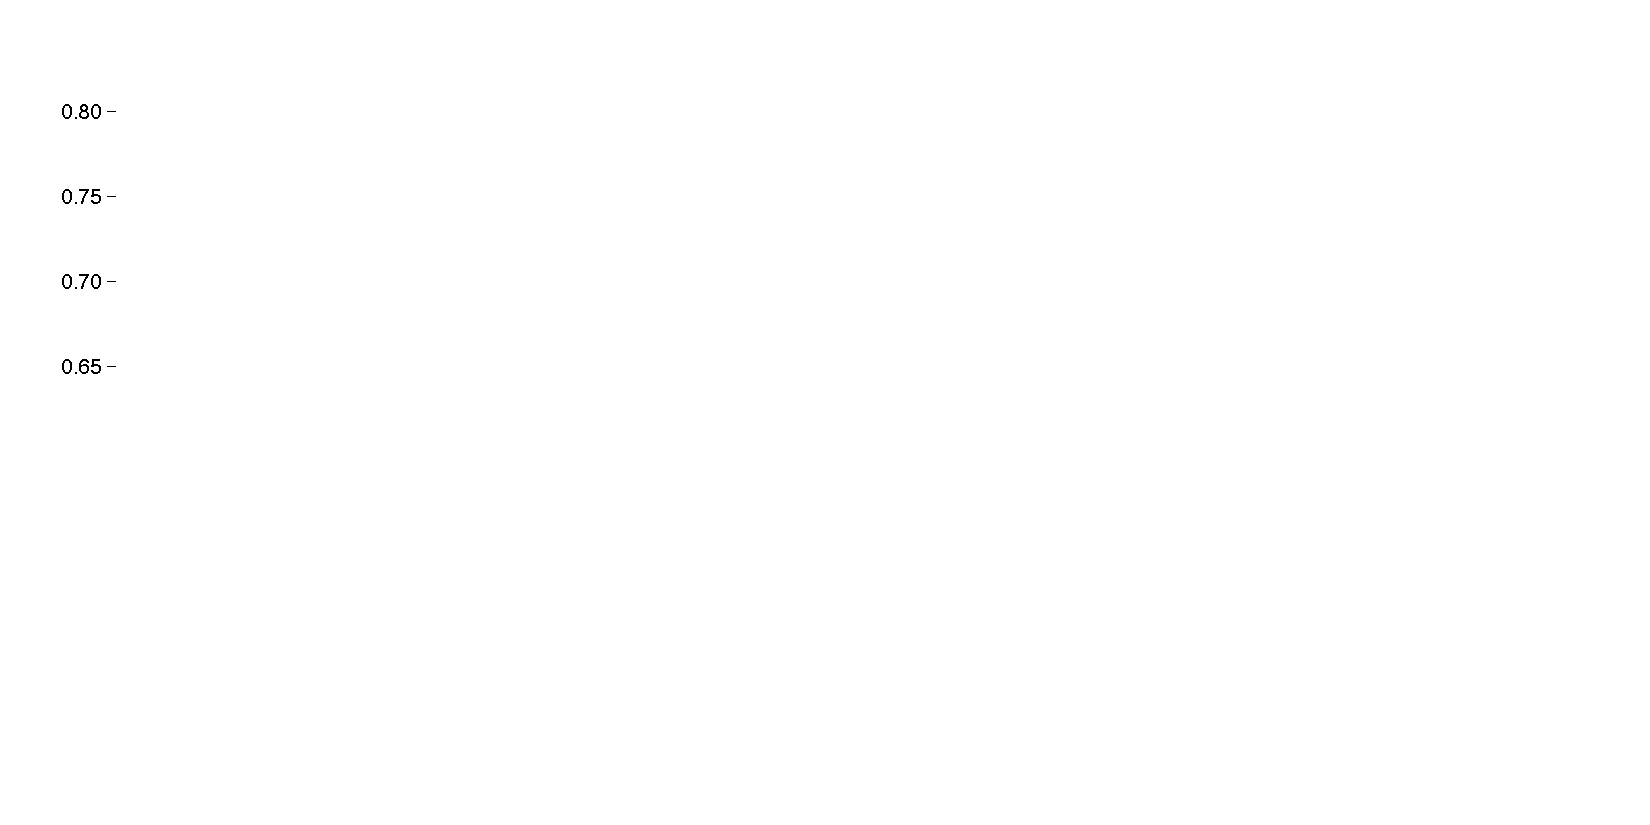
\includegraphics[scale=\graphscale]{reading_tea_leaves/tasks/mp_y}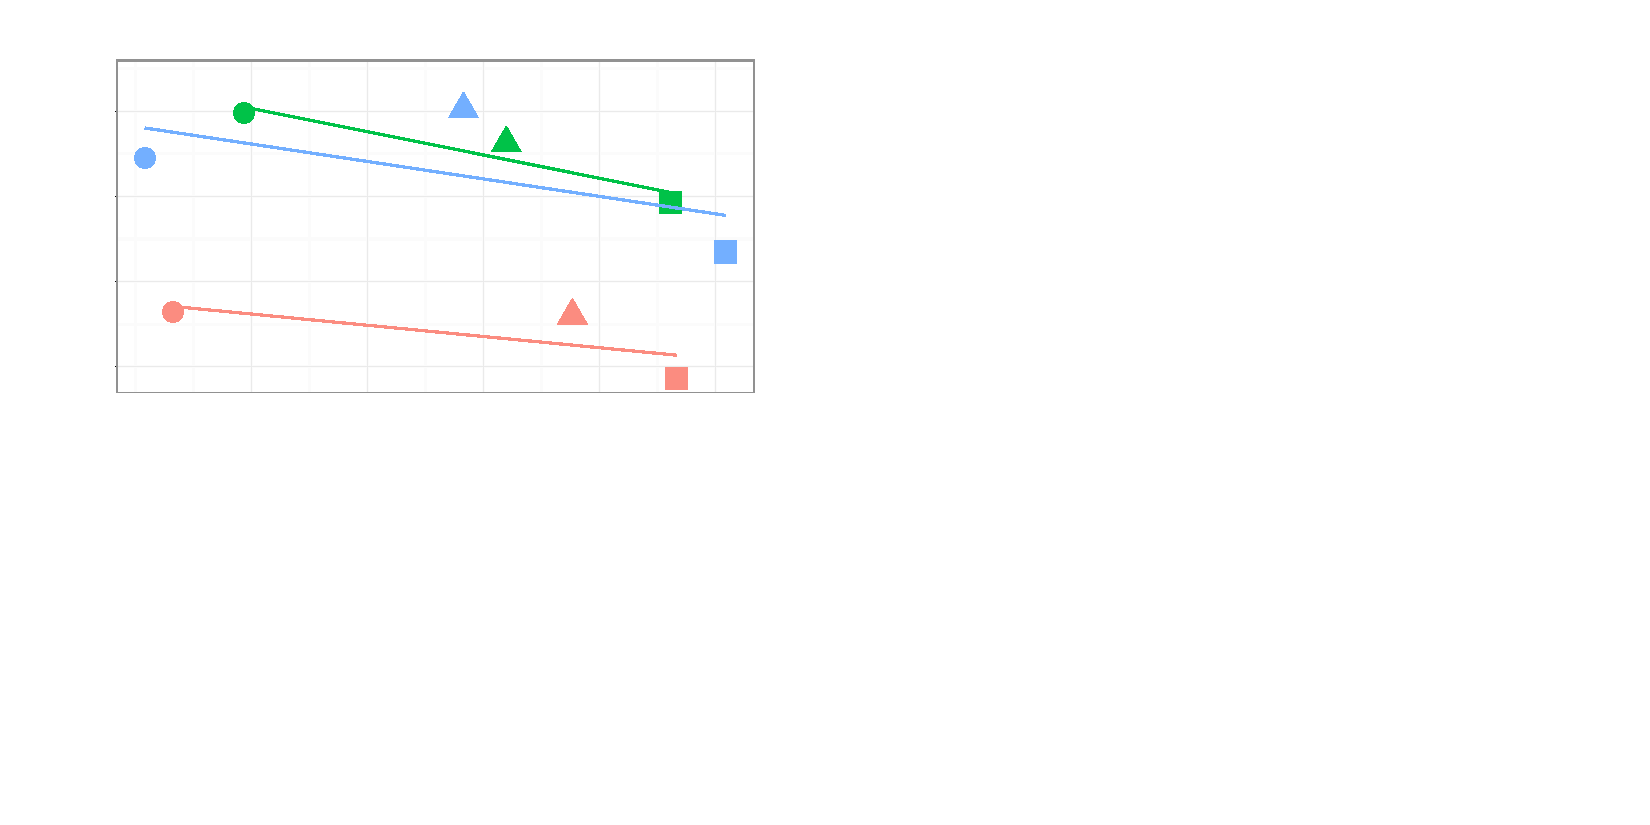
\includegraphics[scale=\graphscale]{reading_tea_leaves/tasks/nyt_mp}\\}
\iflong
  \only<2>{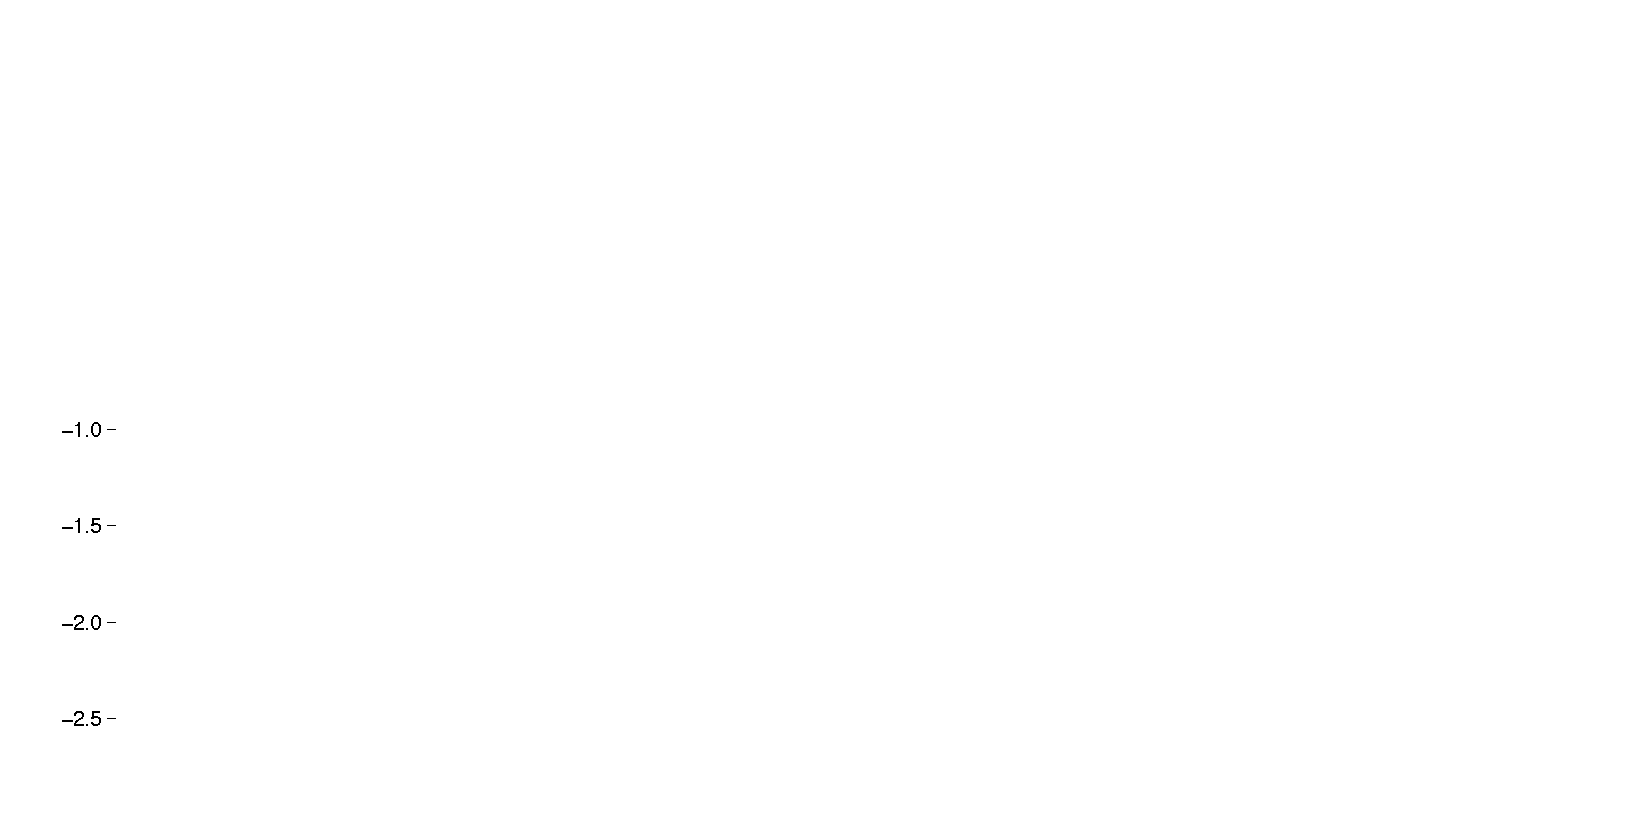
\includegraphics[scale=\graphscale]{reading_tea_leaves/tasks/tlo_y}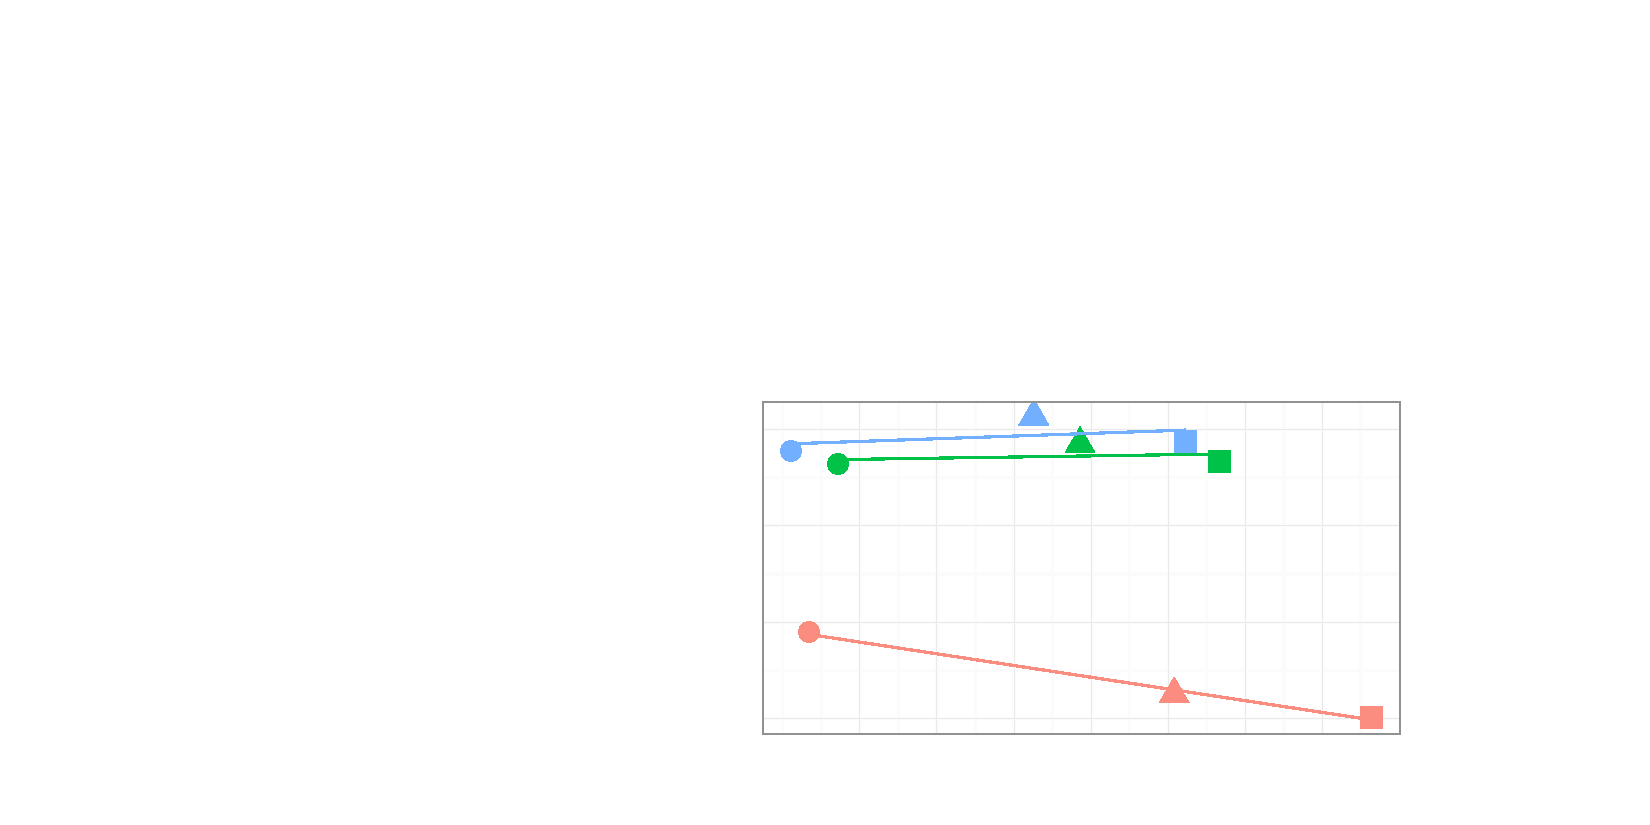
\includegraphics[scale=\graphscale]{reading_tea_leaves/tasks/wiki_tlo}\\}
\fi
  \only<1>{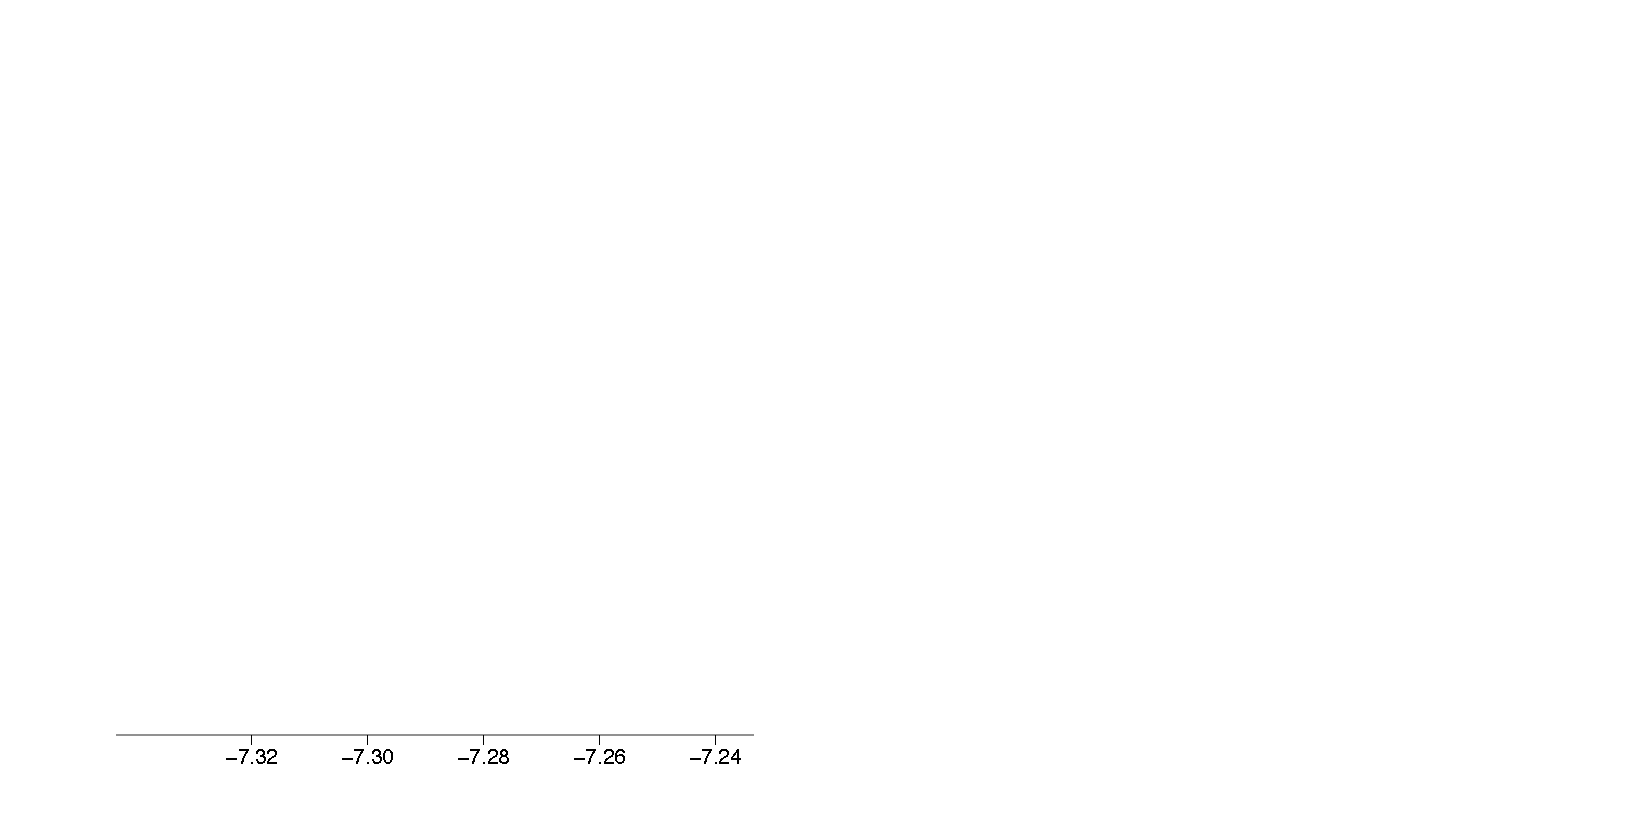
\includegraphics[scale=\graphscale]{reading_tea_leaves/tasks/nyt_x}}
\iflong
  \only<2>{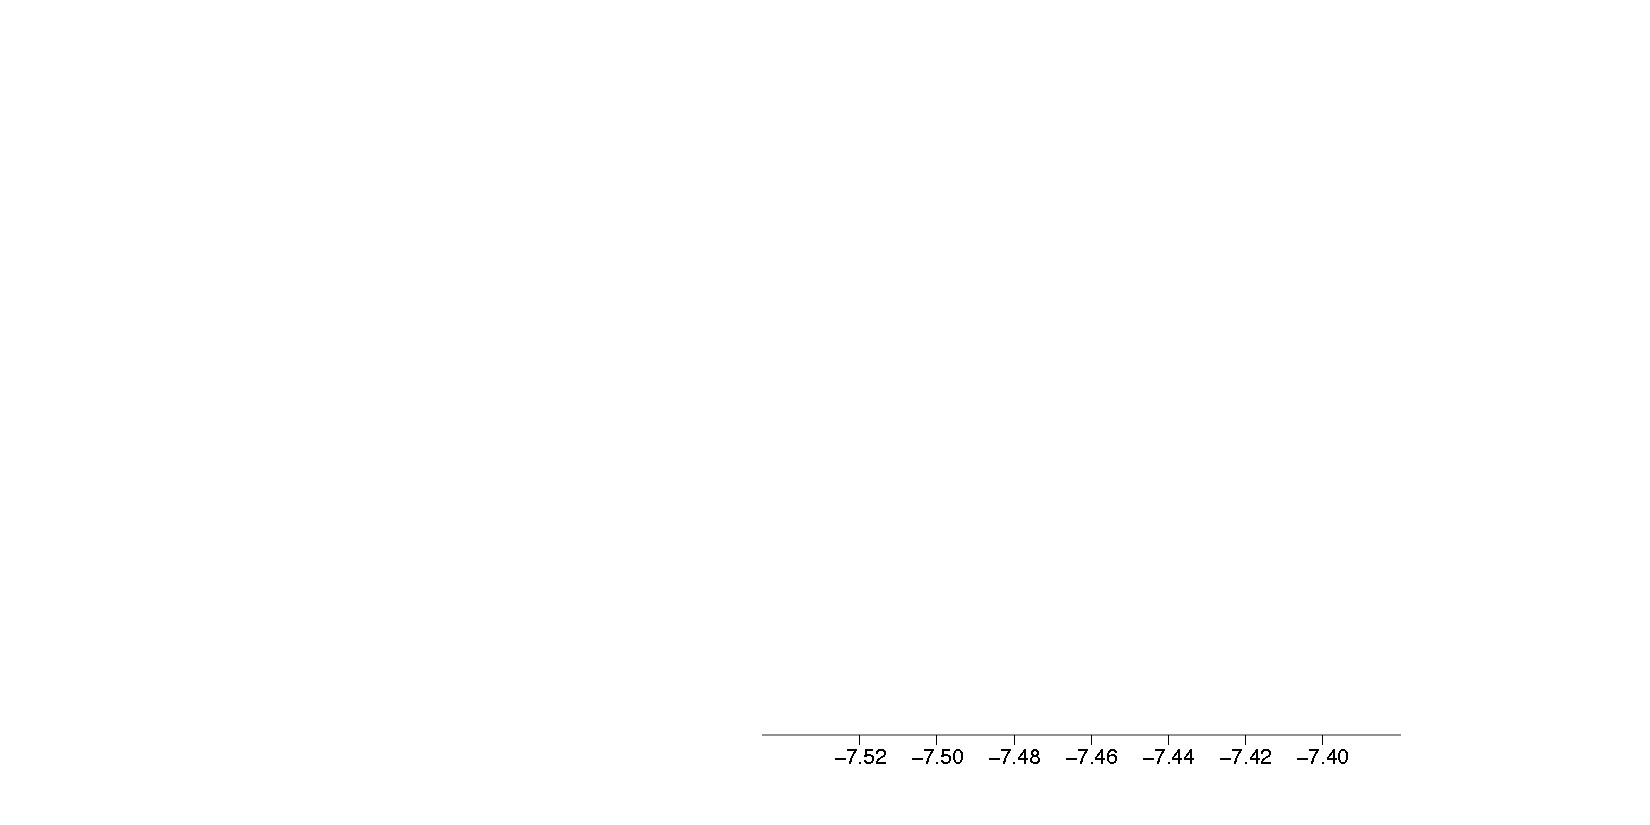
\includegraphics[scale=\graphscale]{reading_tea_leaves/tasks/wiki_x}}
\fi
\end{flushright}
\column{.15\linewidth}
  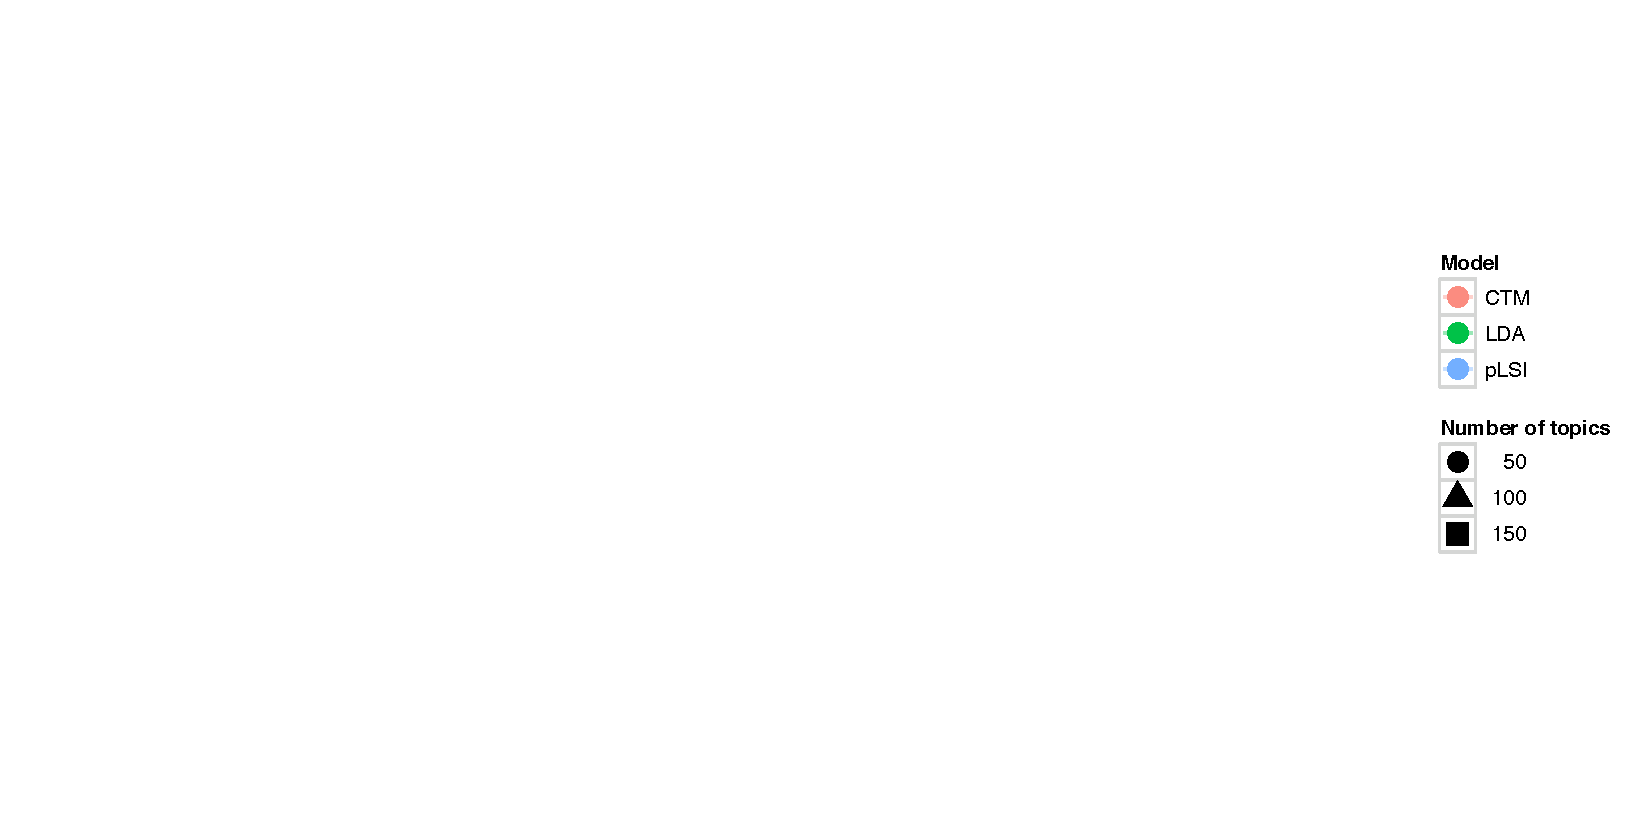
\includegraphics[scale=\graphscale]{reading_tea_leaves/tasks/legend}
\end{columns}
\vspace{-0.75cm}
\begin{center}
  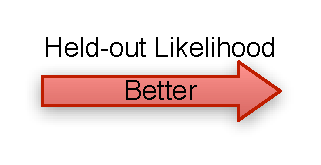
\includegraphics[scale=\graphscale]{reading_tea_leaves/tasks/held-out} \\
\only<1> {within a model, higher likelihood $\not =$ higher interpretability}
\iflong
\only<2> {across models, higher likelihood $\not =$ higher interpretability}
\fi
\end{center}
}

\frame{
\frametitle{Takeaway}
\begin{itemize}
  \item Disconnect between evaluation and use
  \item Means of evaluating an \emph{unsupervised} method
  \item For topic models, direct measurement of interpretability
  \item Surprising relationship between interpretability and likelihood
  \item Measure what you care about
  \end{itemize}
}


